


%%%%%%%%%%%%%%%%%%%%%%%%%%%%%%%%%%%%%%%%%
% Beamer Presentation
% LaTeX Template
% Version 1.0 (10/11/12)
%
% This template has been downloaded from:
% http://www.LaTeXTemplates.com
%
% License:
% CC BY-NC-SA 3.0 (http://creativecommons.org/licenses/by-nc-sa/3.0/)
%
%%%%%%%%%%%%%%%%%%%%%%%%%%%%%%%%%%%%%%%%%

%----------------------------------------------------------------------------------------
%	PACKAGES AND THEMES
%----------------------------------------------------------------------------------------

\documentclass{beamer}

\mode<presentation> {

% The Beamer class comes with a number of default slide themes
% which change the colors and layouts of slides. Below this is a list
% of all the themes, uncomment each in turn to see what they look like.

%\usetheme{default}
%\usetheme{AnnArbor}
%\usetheme{Antibes}
%\usetheme{Bergen}
%\usetheme{Berkeley}
%\usetheme{Berlin}
%\usetheme{Boadilla}
%\usetheme{CambridgeUS}
%\usetheme{Copenhagen}
\usetheme{Darmstadt}
%\usetheme{Dresden}
%\usetheme{Frankfurt}
%\usetheme{Goettingen}
%\usetheme{Hannover}
%\usetheme{Ilmenau}
%\usetheme{JuanLesPins}
%\usetheme{Luebeck}
%\usetheme{Madrid}
%\usetheme{Malmoe}
%\usetheme{Marburg}
%\usetheme{Montpellier}
%\usetheme{PaloAlto}
%\usetheme{Pittsburgh}
%\usetheme{Rochester}
%\usetheme{Singapore}
%\usetheme{Szeged}
%\usetheme{Warsaw}

% As well as themes, the Beamer class has a number of color themes
% for any slide theme. Uncomment each of these in turn to see how it
% changes the colors of your current slide theme.

%\usecolortheme{albatross}
\usecolortheme{beaver}
%\usecolortheme{beetle}
%\usecolortheme{crane}
%\usecolortheme{dolphin}
%\usecolortheme{dove}
%\usecolortheme{fly}
%\usecolortheme{lily}
%\usecolortheme{orchid}
%\usecolortheme{rose}
%\usecolortheme{seagull}
%\usecolortheme{seahorse}
%\usecolortheme{whale}
%\usecolortheme{wolverine}

\setbeamertemplate{footline} % To remove the footer line in all slides uncomment this line
%\setbeamertemplate{footline}[page number] % To replace the footer line in all slides with a simple slide count uncomment this line

\setbeamertemplate{navigation symbols}{} % To remove the navigation symbols from the bottom of all slides uncomment this line
}

\usepackage{graphicx} % Allows including images
\usepackage{booktabs} % Allows the use of \toprule, \midrule and \bottomrule in tables
\usepackage{etex}
\usepackage{listings}
\usepackage{pgfplots}
\usepackage[all]{xy}
\usepackage{multimedia}
\usepackage{media9}
\usepackage[font=Times, timeinterval= 59]{tdclock}
\usetikzlibrary{positioning}
\usetikzlibrary{shapes.geometric}

%----------------------------------------------------------------------------------------
%	TITLE PAGE
%----------------------------------------------------------------------------------------

\title{A Formally Verified Schulze Method} % The short title appears at the bottom of every slide, the full title is only on the title page

%\author{Mukesh Tiwari} % Your name
\author[Mukesh Tiwari]{Mukesh Tiwari\\{\small Supervisors:\newline Dirk Pattinson\newline 
Rajeev Gore\newline Michael Norrish}}
\institute[ANU] % Your institution as it will appear on the bottom of every slide, may be shorthand to save space
{
Australian National University \\[1em] Research School of Computer Science% Your institution for the title page
\medskip
%\textit{john@smith.com} % Your email address
}
\date{12 September, 2019} % Date, can be changed to a custom date


\begin{document}


\defverbatim[colored]\lstf{
\begin{lstlisting}[language=haskell, basicstyle=\ttfamily\scriptsize, commentstyle=\color{red}\ttfamily]
{- Propositional Path -}
Inductive Path (k: Z) : node -> node -> Prop :=     
| unit c d : node_strength c d >= k -> Path k c d    
| cons  c d e : 
   node_strength c d >= k -> Path k d e -> Path k c e.
   
{- Notion of winner at prop level -}    
Definition wins_prop (c: node) := 
  forall d : node, exists k : Z,     
   Path k c d /\ 
   (forall l, Path l d c -> l <= k).   

{- Notion of loser at prop level -}
Definition loses_prop (c : node) := 
  exists k: Z, exists  d: node,     
   Path k d c /\ 
   (forall l, Path l c d -> l < k).
\end{lstlisting}}

\defverbatim[colored]\lsts{
\begin{lstlisting}[language=haskell, basicstyle=\ttfamily\scriptsize]

Definition marg_lt (k : Z) (p : (cand * cand)) :=
	Zlt_bool (marg (fst p) (snd p)) k.

Definition W (k:Z) (p:cand * cand -> bool) (x:cand * cand) :=     
 andb (marg_lt k x)       
 (forallb (fun m => 
   orb (marg_lt k (fst x, m)) 
       (p (m, snd x))) cand_all).
 
Definition coclosed (k:Z) 
 (f:(cand * cand) -> bool) :=     
  forall x, f x = true -> W k f x = true.   
 
    
\end{lstlisting}}


\defverbatim[colored]\lstt{
\begin{lstlisting}[language=haskell,commentstyle=\color{red}\ttfamily, basicstyle=\ttfamily\scriptsize ]
{- Type level Path -}
Inductive PathT (k: Z) : cand -> cand -> Type :=   
| unitT :forall c d, 
   marg c d >= k -> PathT k c d   
| consT :forall c d e,
   marg c d >= k -> PathT k d e -> PathT k c e.

{- Notion of winner at type level -} 
Definition wins_type c := 
 forall d : cand, existsT (k : Z),     
  (PathT k c d * existsT f,       
  f (d, c) = true /\ coclosed (k + 1) f)).   

{- Notion of loser at type level -}
Definition loses_type (c : cand) := 
 existsT (k : Z) (d : cand),     
  (PathT k d c * existsT f,       
  f (c, d) = true /\ coclosed k f)).
  
Lemma wins_type_prop : forall c, wins_type c -> wins_prop c.  
Lemma wins_prop_type : forall c, wins_prop c -> wins_type c.
\end{lstlisting}
}


\defverbatim[colored]\lstfourth{
\begin{lstlisting}[language=haskell, basicstyle=\ttfamily\tiny, commentstyle=\color{red}\ttfamily]
Inductive State: Type :=     
| partial: (list ballot * list ballot)  -> (cand -> cand -> Z) -> State     
| winners: (cand -> bool) ->  State.

{- Different states of counting -}
Inductive Count (bs : list ballot) : State -> Type :=     
| ax us m : us=bs -> (forall c d, m c d = 0) -> 
   Count bs (partial (us, []) m)            
| cvalid u us m nm inbs : 
   Count bs (partial (u :: us, inbs) m) -> 
   (forall c, u c > 0) -> 
   (forall c d : cand, 
     (u c < u d -> nm c d = m c d + 1) /\                                           
     (u c = u d -> nm c d = m c d)     /\                                    
     (u c > u d -> nm c d = m c d - 1)) ->                                
   Count bs (partial (us, inbs) nm)
| cinvalid u us m inbs : 
   Count bs (partial (u :: us, inbs) m) ->
   (exists c, u c = 0) -> Count bs (partial (us, u :: inbs) m)     
| fin m inbs w (d : (forall c, (wins_type m c) + (loses_type m c))):
   Count bs (partial ([], inbs) m) -> 
   (forall c, w c = true <-> (exists x, d c = inl x)) ->         
   (forall c, w c = false <-> (exists x, d c = inr x)) ->         
   Count bs (winners w).    
\end{lstlisting}
}


\defverbatim[colored]\lstfifth{
\begin{lstlisting}[language=haskell, basicstyle=\ttfamily\tiny]
Theorem schulze_winners: forall (bs : list ballot),     
  existsT (f : cand -> bool) (p : Count bs (winners f)), True.
  
V: [A1 B2 C3,..], I:  [], M: [AB:0 AC:0 BC:0]
---------------------------------------------
V: [A1 B2 C3,..], I:  [], M: [AB:1 AC:1 BC:1]
---------------------------------------------
             . . .
---------------------------------------------
V: [A2 B3 C1], I:  [], M: [AB:2 AC:0 BC:6]
------------------------------------------
V: [], I: [], M: [AB:3 AC:-1 BC:5]
----------------------------------
winning: A
   for B: path A -> B of strenght 3, 4-coclosed set:
     [(A,A),(B,A),(B,B),(C,A),(C,B),(C,C)]
   for C: path A -> B -> C of strenght 3, 4-coclosed set:
     [(A,A),(B,A),(B,B),(C,A),(C,B),(C,C)] 
losing: B
   exists A: path A -> B of strength 3, 3-coclosed set:
     [(A,A),(B,A),(B,B),(C,A),(C,B),(C,C)]
losing: C
   exists A: path A -> B -> C of strength 3, 3-coclosed set:
     [(A,A),(B,A),(B,B),(C,A),(C,B),(C,C)]  
\end{lstlisting}
}

\defverbatim[colored]\lstsix{
\begin{lstlisting}[language=haskell, basicstyle=\ttfamily\tiny]
Inductive HState: Type :=
 | hpartial: (list eballot * list eballot)  -> (cand -> cand -> Z) -> HState 
 | hdecrypt: (cand -> cand -> Z) -> HState
 | winners: (cand -> bool) -> HState.	
\end{lstlisting}
}

\defverbatim[colored]\lstseven{
\begin{lstlisting}[language=haskell, basicstyle=\ttfamily\tiny]
Inductive HCount (bs : list eballot) : HState -> Type :=
 | ax us (m : cand -> cand -> Z) (ev : cand -> cand -> Z): 
      us = bs -> (forall c d, enc 0 (ev c d) = m c d) -> 
      HCount bs (hpartial (us, []) m)

 | cvalid u us m nm inbs (v : cand -> cand -> Z) (p : Zkp u v) 
          (b : cand -> cand -> Z)
          (ev : cand -> cand -> Z) :
          HCount bs (hpartial (u :: us, inbs) m) -> 
          (check_zkp u v (p : Zkp u v) = true) -> 
          (forall c d, enc (b c d) (ev c d) = v c d) ->
          valid b ->
          (forall c d, nm c d = m c d  + u c d) ->
          HCount bs (hpartial (us, inbs) nm)
  
 | cinvalid u us m inbs (v : cand -> cand -> Z) (p : Zkp u v) 
            (b : cand -> cand -> Z)
            (ev : cand -> cand -> Z) : 
            HCount bs (hpartial (u :: us, inbs) m) ->
            (check_zkp u v p = true) -> 
            (forall c d, enc (b c d) (ev c d) = v c d) -> 
            invalid b  -> 
            HCount bs (hpartial (us, u :: inbs) m)

 
\end{lstlisting}
}
\defverbatim[colored]\lsteight{
\begin{lstlisting}[language=haskell, basicstyle=\ttfamily\tiny]

| cderypt inbs m ev dm : HCount bs (hpartial ([], inbs) m) -> 
           (forall c d, enc (m c d) (ev c d) = dm c d) ->
           HCount bs (hdecrypt dm)

 | fin dm w (d : (forall c, (wins_type dm c) + (loses_type dm c))) :
        HCount bs (hdecrypt dm) -> 
        (forall c, w c = true <-> (exists x, d c = inl x)) ->
        (forall c, w c = false <-> (exists x, d c = inr x)) ->
        HCount bs (winners w).	
        
\end{lstlisting}
}

 
\defverbatim[colored]\lstnineth{
\begin{lstlisting}[language=haskell, basicstyle=\ttfamily\tiny]
V: [A3 B1 C2 D4,..], I: [], M: [AB:0 AC:0 AD:0 BC:0 BD:0 CD:0]
--------------------------------------------------------------
V: [A1 B0 C4 D3,..], I: [], M: [AB:-1 AC:-1 AD:1 BC:1 BD:1 CD:1]
----------------------------------------------------------------
V: [A3 B1 C2 D4,..], I: [A1 B0 C4 D3], M: [AB:-1 AC:-1 AD:1 BC:1 BD:1 CD:1]
---------------------------------------------------------------------------
                     . . .
----------------------------------------------------------------------
V: [A1 B3 C2 D4], I: [A1 B0 C4 D3], M: [AB:2 AC:2 AD:8 BC:5 BD:8 CD:8]
----------------------------------------------------------------------
V: [], I: [A1 B0 C4 D3], M: [AB:3 AC:3 AD:9 BC:4 BD:9 CD:9]
-----------------------------------------------------------
winning: A
  for B: path A --> B of strength 3, 4-coclosed set: 
    [(B,A),(C,A),(C,B),(D,A),(D,B),(D,C)]
  for C: path A --> C of strength 3, 4-coclosed set:
    [(B,A),(C,A),(C,B),(D,A),(D,B),(D,C)]
  for D: path A --> D of strength 9, 10-coclosed set:
    [(D,A),(D,B),(D,C)]
losing: B
  exists A: path A --> B of strength 3, 3-coclosed set:
    [(A,A),(B,A),(B,B),(C,A),(C,B),(C,C),(D,A),(D,B),(D,C),(D,D)]
losing: C
  exists A: path A --> C of strength 3, 3-coclosed set:
    [(A,A),(B,A),(B,B),(C,A),(C,B),(C,C),(D,A),(D,B),(D,C),(D,D)]
losing: D
  exists A: path A --> D of strength 9, 9-coclosed set:
    [(A,A),(A,B),(A,C),(B,A),(B,B),(B,C),(C,A),(C,B),(C,C),(D,A),(D,B),
     (D,C),(D,D)]
\end{lstlisting}
}       

\defverbatim[colored]\lsttenth{
\begin{lstlisting}[language=haskell, basicstyle=\ttfamily\tiny]

Inductive Path (k: Z) : cand -> cand -> Prop :=     
| unit c d : marg c d >= k -> Path k c d    
| cons  c d e : 
   marg c d >= k -> Path k d e -> Path k c e.  
        
\end{lstlisting}
}

\defverbatim[colored]\lsteleven{
\begin{lstlisting}[language=haskell, basicstyle=\ttfamily\scriptsize]

Lemma iterated_marg_fp: forall (c d : cand) (n : nat),
      M n c d <= M (length cand_all) c d.

Lemma wins_prop_iterated_marg (c : cand) : wins_prop c ->
      forall d, M (length cand_all) d c <= M (length cand_all) c d.

Lemma iterated_marg_wins_type (c : cand) : (forall d,
      M (length cand_all) d c <= M (length cand_all) c d) ->
      wins_type c.

        
\end{lstlisting}
} 

\defverbatim[colored]\lsttwelve{
\begin{lstlisting}[language=haskell, basicstyle=\ttfamily\scriptsize]
Theorem schulze_winners: forall (bs : list ballot),     
  existsT (f : cand -> bool) (p : Count bs (winners f)), True.
  

\end{lstlisting}
}



\defverbatim[colored]\lstthirteen{
\begin{lstlisting}[language=haskell, basicstyle=\ttfamily\tiny]
Definition plaintext := Z.
Definition ciphertext := (Z * Z)%type. 


    (* ballot is plain text value *)
Definition ballot := cand -> cand -> plaintext.
    (* eballot is encrypted value *)
Definition eballot := cand -> cand -> ciphertext.

    

Inductive HState: Type :=
 | hpartial: (list eballot * list eballot)  -> (cand -> cand -> ciphertext) -> HState
 | hdecrypt: (cand -> cand -> plaintext) -> HState
 | winners: (cand -> bool) -> HState.

    (* Public key and private key are integers *)
Definition Pubkey := Z.
Definition Prikey := Z.

    (* private and public key *)
Variable privatekey : Prikey.
Variable publickey : Pubkey.

\end{lstlisting}
}

\defverbatim[colored]\lstfourteen{
\begin{lstlisting}[language=haskell, basicstyle=\ttfamily\tiny]
	(* This function will be realized by Elgamal Encryption.
 		Enc_Pk (m, r) = (g^r, g^m * h^r) *)
Variable encrypt_ballot : Pubkey -> ballot ->  eballot.

    (* This function will be realized by Elgamal Decryption
       which takes encrypted message (c1, c2), private key
       and outputs the plaintext message *)
Variable decrypt_ballot : Prikey -> eballot -> ballot.

    (* This function takes encrypted ballot and returns
       permuted encrypted ballot with zero knowledge proof.
       For the moment, zero knowledge proof is assumed to
       be of type Z *)
Variable permute_encrypted_ballot : eballot ->  eballot * Z.

    (* This function takes encrypted margin function and encrypted ballot
       and multiply them pointwise. *)
Variable homomorphic_add_eballots :
      (cand -> cand -> ciphertext) ->
      eballot -> (cand -> cand -> ciphertext).

    (* This function show that ciphertext (c_1, c_2) is indeed the
       the encryption of message m under zero knowledge proof. *)

Variable zero_knowledge_decryption : plaintext -> ciphertext -> Z -> bool.

\end{lstlisting}
}


\defverbatim[colored]\lstfifteen{
\begin{lstlisting}[language=haskell, basicstyle=\ttfamily\tiny]
	(* This function is takes u, v and val where permute u = (v, val)
       and return true or false *)
Variable certify_permuted_ballots : eballot -> eballot -> Z -> bool.

Inductive HCount (bs : list eballot) : HState -> Type :=
    (* start of counting *)
 | ax us (m : cand -> cand -> ciphertext) (zkpdecm : Z)
         (* for the moment we are assuming it as integer, but it is zero knowledge proof 
            about m zero encrypted matrix *) :
        us = bs (* We start from uncounted ballots *) ->
        (* (forall c d, zero_knowledge_decryption 0 (m c d) zkpdecm = true) ->
           This is useless, because this statement is not proved in coq, but 
           will run at execution of extracted code, and should return true if 
           m is encrypted zero matrix. It helps to keep track about the
           Honest decryption proof that m is encryption of zero matrix *)
        HCount bs (hpartial (us, []) m)
    (* Valid Ballot *)
 | cvalid u (v : eballot) b (zkppermuv : Z) (zkpdecv : Z) us m nm inbs :
        HCount bs (hpartial (u :: us, inbs) m) ->
        valid cand (fun c d => b c d = 1) -> 
        (* u -> v -> b.
           b is honest decryption of v proved under zero knowledge proof, zkpdecv, 
           data structure which is Z for the moment. 
           zkppermuv is zero knowledge proof data structure about v being
           permutation of u. b is valid ballot and using the lemma 
           perm_presv_validity, it follows to decryption of u.
           permute_encrypted_ballot u = (v, zkp) and 
           ceritify_permuted_ballots u v zkp = true *)
        (* Proof that new margin is encrypted sum 
        (forall c d, nm c d = homomorphic_add_eballots m u c d) -> *)
        HCount bs (hpartial (us, inbs) nm)
\end{lstlisting}
}
\defverbatim[colored]\lstsixteen{
\begin{lstlisting}[language=haskell, basicstyle=\ttfamily\tiny]
    (* Invalid ballot *)
 | cinvalid u (v : eballot) b (zkppermuv : Z) (zkpdecv : Z) us m inbs :
        HCount bs (hpartial (u :: us, inbs) m) ->
        ~valid cand (fun c d => b c d = 1) -> 
        (* u -> v -> b.
           b is honest decryption of v proved under zero knowledge proof, zkpdecv, 
           data structure which is Z for the moment. 
           zkppermuv is zero knowledge proof data structure about v being
           permutation of u. b is invalid ballot and using the lemma
           not_perm_persv_validity, it follows to decryption of u. *)
        HCount bs (hpartial (us, u :: inbs) m) 
    (* Decrypt the margin function at this point with proof that it is
        honest decryption *)
 | cdecrypt inbs m dm (zkpdecm : Z):
        HCount bs (hpartial ([], inbs) m) ->
        (* proof of honest decryption. zkpdecm is zero knowledge proof datastructure 
           which proves that dm is decryption of m under zero knowledge proof. 
        (forall c d, zero_knowledge_dec (dm c d) (m c d) zkpdecm = true) -> *)
        HCount bs (hdecrypt dm)
    (* Compute the winner *)
 | fin dm w (d : (forall c, (wins_type dm c) + (loses_type dm c))) :
        HCount bs (hdecrypt dm) ->
        (forall c, w c = true <-> (exists x, d c = inl x)) ->
        (forall c, w c = false <-> (exists x, d c = inr x)) ->
        HCount bs (winners w). 

\end{lstlisting}
}

\defverbatim[colored]\lstseventeen{
\begin{lstlisting}[language=haskell, basicstyle=\ttfamily\tiny]
(* Definition of validity *)
Definition valid (A : Type) (P : A -> A -> Prop) := 
	exists (f : A -> nat), forall (c d : A), P c d <-> (f c < f d)%nat.

Lemma decidable_valid
     : forall (A : Type) (P : A -> A -> Prop),
       (forall c d : A, {c = d} + {c <> d}) ->
       (forall c d : A, {P c d} + {~ P c d}) -> 
       finite A -> {valid A P} + {~ valid A P}
       
Lemma perm_presv_validity :
  	 forall (A : Type) (P : A -> A -> Prop)
         (Adec : forall (c d : A), {c = d} + {c <> d})
         (Pdec : forall c d, {P c d} + {~P c d}) (sig : A -> A)
         (Hsig : Bijective sig), 
		 valid A P <-> valid A (perm A P sig).	

Lemma not_perm_persv_validity :
  	 forall (A : Type) (P : A -> A -> Prop)
         (Adec : forall (c d : A), {c = d} + {c <> d})
         (Pdec : forall c d, {P c d} + {~P c d}) (sig : A -> A)
         (Hsig : Bijective sig),
		~valid A P <-> ~valid A (perm A P sig).
\end{lstlisting}
}

\defverbatim[colored]\lsteighteen{
\begin{lstlisting}[language=haskell, basicstyle=\ttfamily\scriptsize, commentstyle=\color{red}\ttfamily]

{- Natural Number Definition-}
Inductive nat :=
| O : nat
| Suc : nat -> nat.

{- Addition on Natural Numbers -}
Fixpoint add (n m : nat) : nat :=
  match n with
  | O => m
  | Suc n' => Suc (add n' m)
  end.

{- Commutative Property  -}
Theorem add_commute : forall (n m : nat), add n m = add m n.
Proof.
  (* proof terms omitted *)
Qed.

\end{lstlisting}
}

\frame{\titlepage}
%\section[Table of contents]{}
%\frame{\frametitle{Table of contents}\tableofcontents[sections={2-3}]}
%\frame{\frametitle{Table of contents...}\tableofcontents[sections={4}]}
%\frame{\frametitle{Table of contents...}\tableofcontents[sections={5-6}]}

%\section{Introduction}

%\begin{frame}
%\frametitle{Electronic Voting}
%\includegraphics[scale=0.20]{Electronic_voting_1.png}
%\end{frame}
%
%\begin{frame}
%\frametitle{Electronic Voting}
%\includegraphics[scale=0.20]{Electronic_voting_2.png}
%\end{frame}

\begin{frame}
\frametitle{Talk Outline}
\begin{itemize}
%\item Promise
\item Background
\item Motivation
\item Schulze Voting as Evidence Carrying Computation
\item Scaling it to count millions ballot
\item Verifiable Homomorphic Tallying for the Schulze Vote Counting Scheme
\item Certificate : Verifying Elections Formally
\item Machine Checked Properties 
\item Contribution
\item Future Work
\end{itemize}
\end{frame}

%
%\begin{frame}
%\frametitle{Introduction}
%{Free and fair elections are impossible without
%\textbf{Privacy, Verifiability} and \textbf{Correctness}. However, 
%it is almost next to impossible to achieve all three at the same time.}
%
%\end{frame}


\begin{frame}
\frametitle{Background}
{Let me take you back in time and imagine that 
we in 1855. We are going to pub to cast our ballot for a democratic election. 
In the pub, there is counter hanging on wall which shows how many votes 
so far the running  candidates have. 
We raise our hand in the public for the candidate which offers us
beer or money or whatever you like. Everyone sees us to whom we 
voted and the person at counter increments the votes for 
that corresponding candidate}

{Election held in 1855 in Victoria, Australia 
	  was conducted in pub!}
\begin{figure}
	\begin{center}
	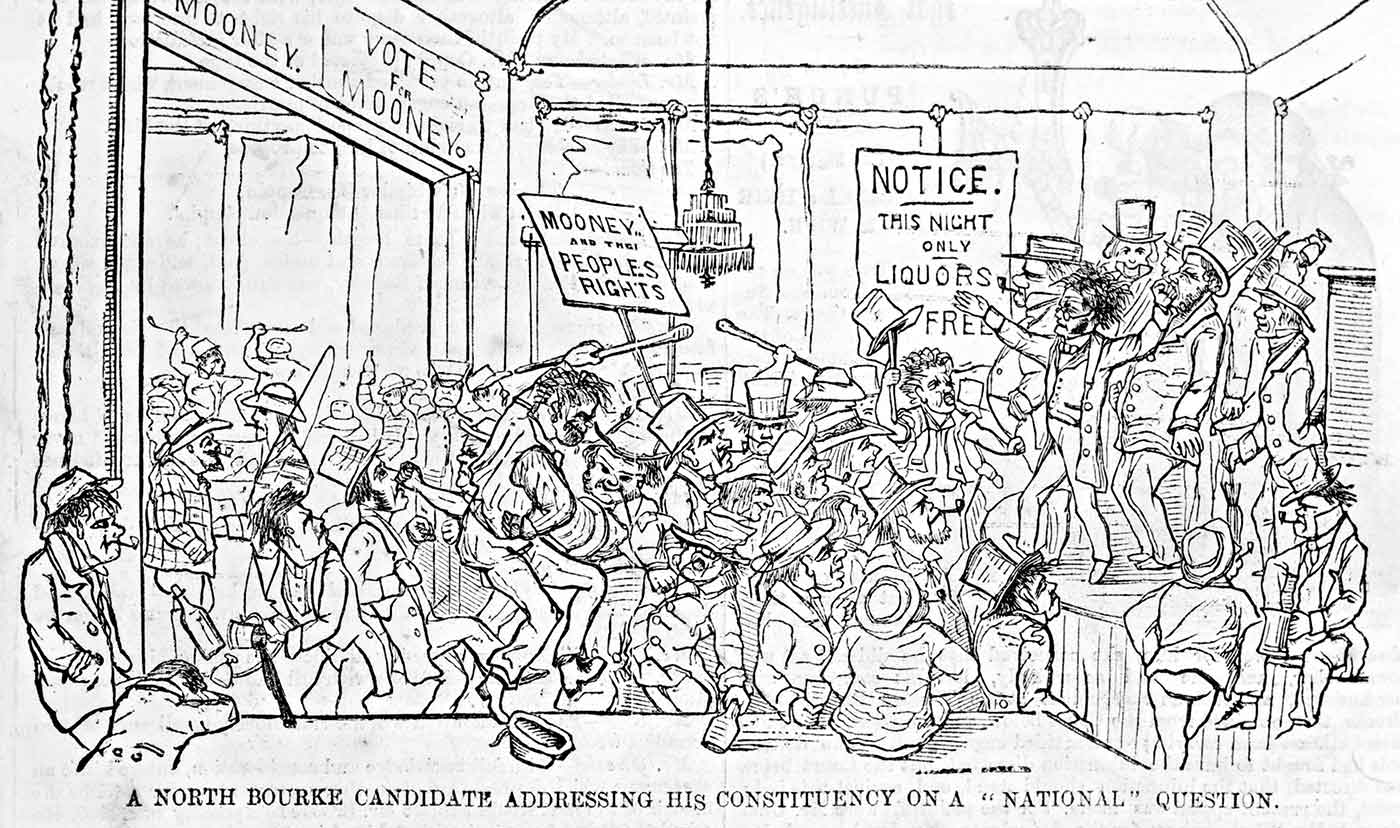
\includegraphics[scale=0.20]{NorthBourke.jpg}
	\end{center}
  \end{figure}   
%{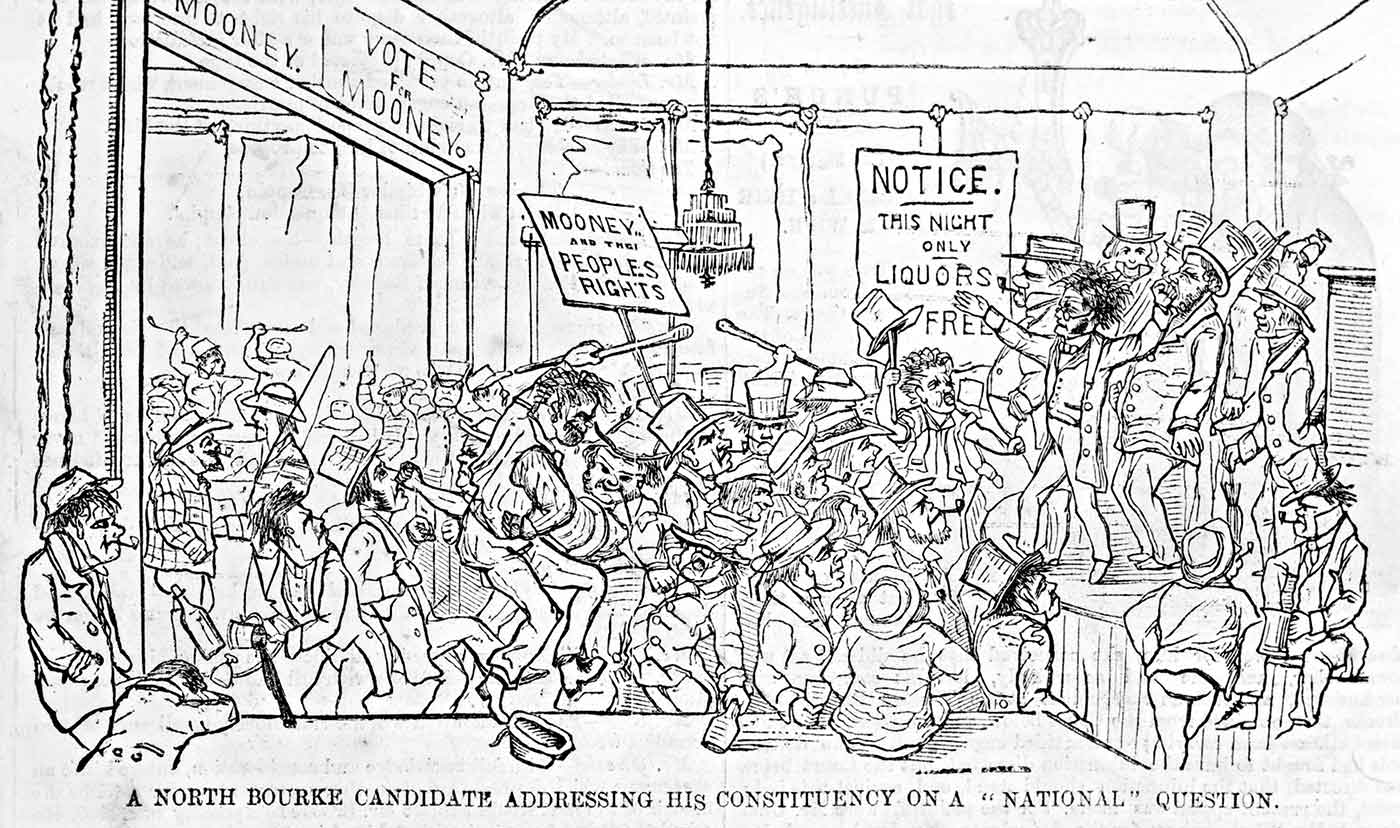
\includegraphics[width=0.50\textwidth]{NorthBourke.jpg}}
\end{frame}

\begin{frame}
\frametitle{Background}
\begin{itemize}[]
\item Pros 
\begin{itemize}
\item<.-> Correctness
\item Verifiability
\item Free Beer
\end{itemize}
\item Cons
\begin{itemize}
\item<.-> Corruption
\item Intimidation
\item Violence
\item Unfair (women and poor were not allowed to even vote)
\end{itemize}
\end{itemize}
\end{frame}


%\begin{frame}
%  \frametitle{Embed this video https://www.youtube.com/watch?v=bWwR2CUNudA}
%      \begin{tikzpicture}[remember picture,overlay]
%         \node[anchor=south west, inner sep=0pt] at (current page.south west) {%
%           \movie[height = \paperheight, width = \paperwidth, poster, showcontrols] {}{DRS2.mp4}%
%         };
%      \end{tikzpicture}
%  \end{frame}
 
 
   
\begin{frame}
\frametitle{Background}
{In order to tackle to the various problems, Australians introduce 
 secret ballot. You go to a secluded place and vote your favourite candidate without 
 anyone knowing. 2019 Election, NSW, Australia}
\begin{figure}
	\begin{center}
	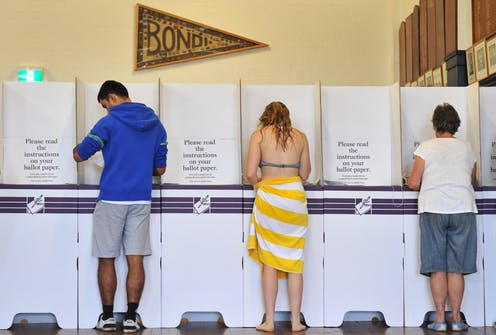
\includegraphics[scale=0.50]{image-20160525-25209-cn3ftj.jpg}
	\end{center}
  \end{figure}   
\end{frame}


\begin{frame}
\frametitle{Background}
\begin{itemize}[]
\item Pros 
\begin{itemize}
\item<.-> Privacy 
\item Verifiability
\item Correctness
\end{itemize}
\item Cons
\begin{itemize}
\item Sadly, no free beer
\end{itemize}
\end{itemize}
\end{frame}

%
%\begin{frame}
%\frametitle{Background}
%{Now that we have privacy, how do we make sure that the counting 
%is correct and process is verifiable? Enter Scrutineers}
%\begin{figure}
%	\begin{center}
%	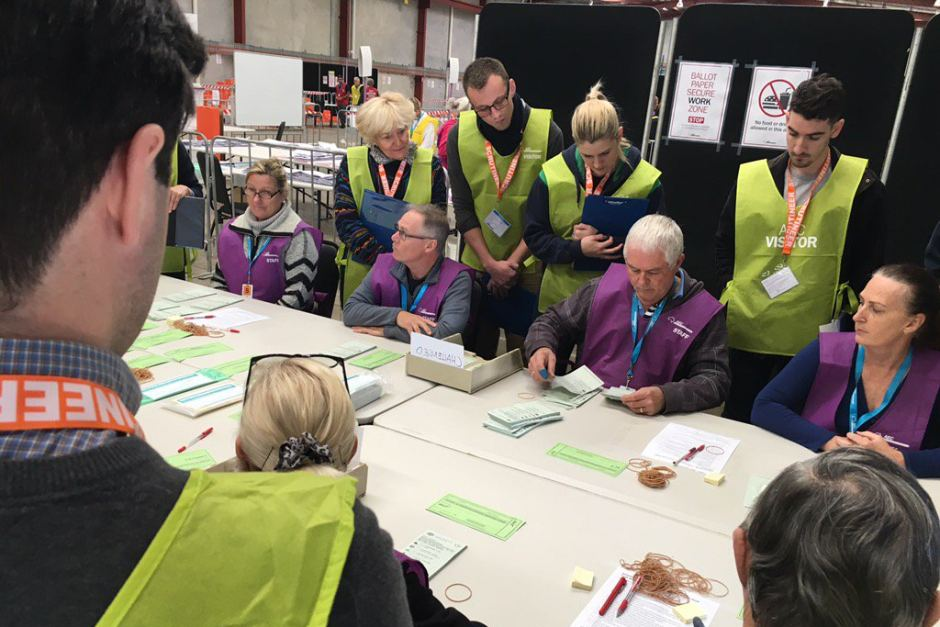
\includegraphics[scale=0.15]{scrutneers.jpg}
%	\end{center}
%  \end{figure}  
%\end{frame}


\begin{frame}
\frametitle{Background}
{Slow for big countries like India}
\begin{figure}
	\begin{center}
	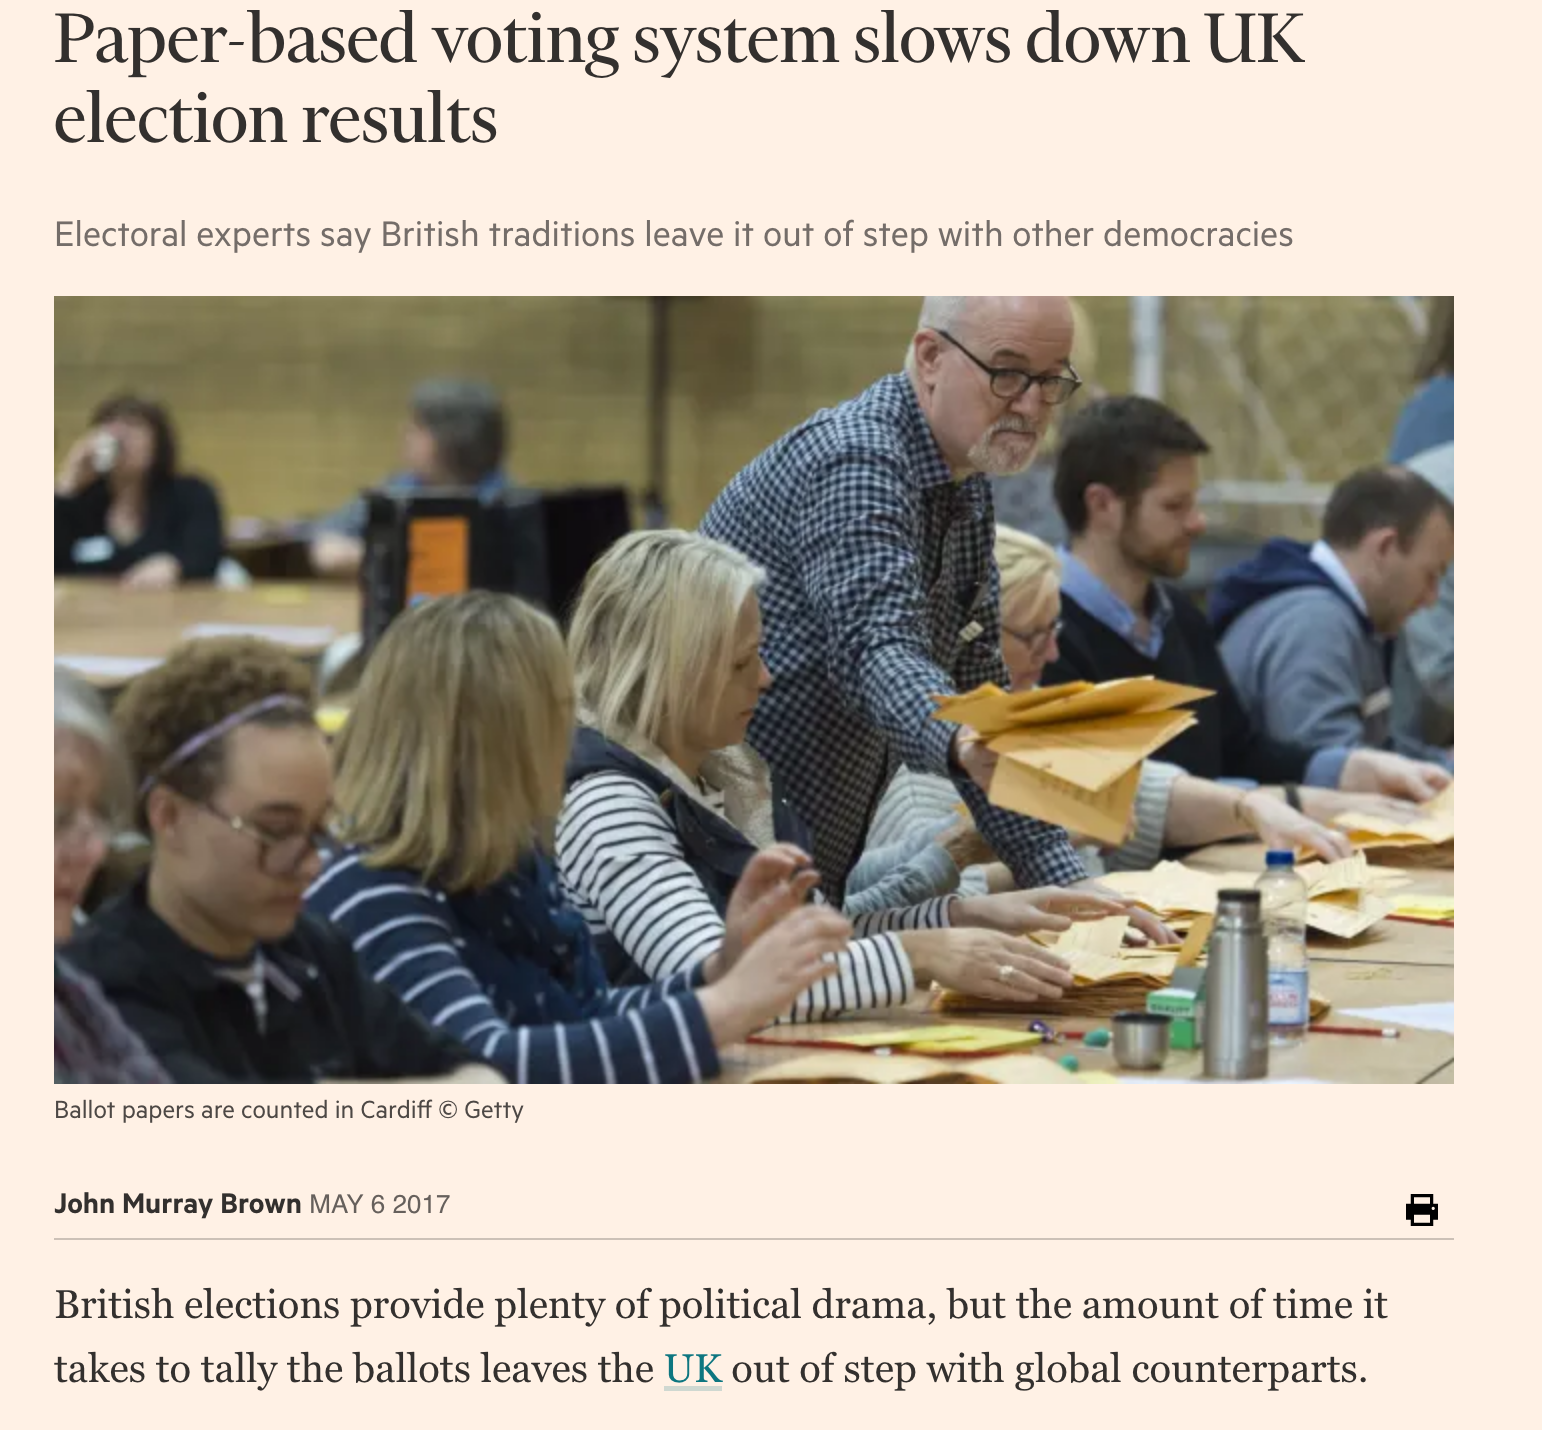
\includegraphics[scale=0.25]{uk-election.png}
	\end{center}
  \end{figure} 
\end{frame}

\begin{frame}
\frametitle{Background}
{Costly}
\begin{figure}
	\begin{center}
	
\includegraphics[scale=0.25]{re-election.png}
	\end{center}
  \end{figure} 
\end{frame}


\begin{frame}
\frametitle{Background}
{Logistic challenge for sparsely populated countries Australia }
\begin{figure}
	\begin{center}
	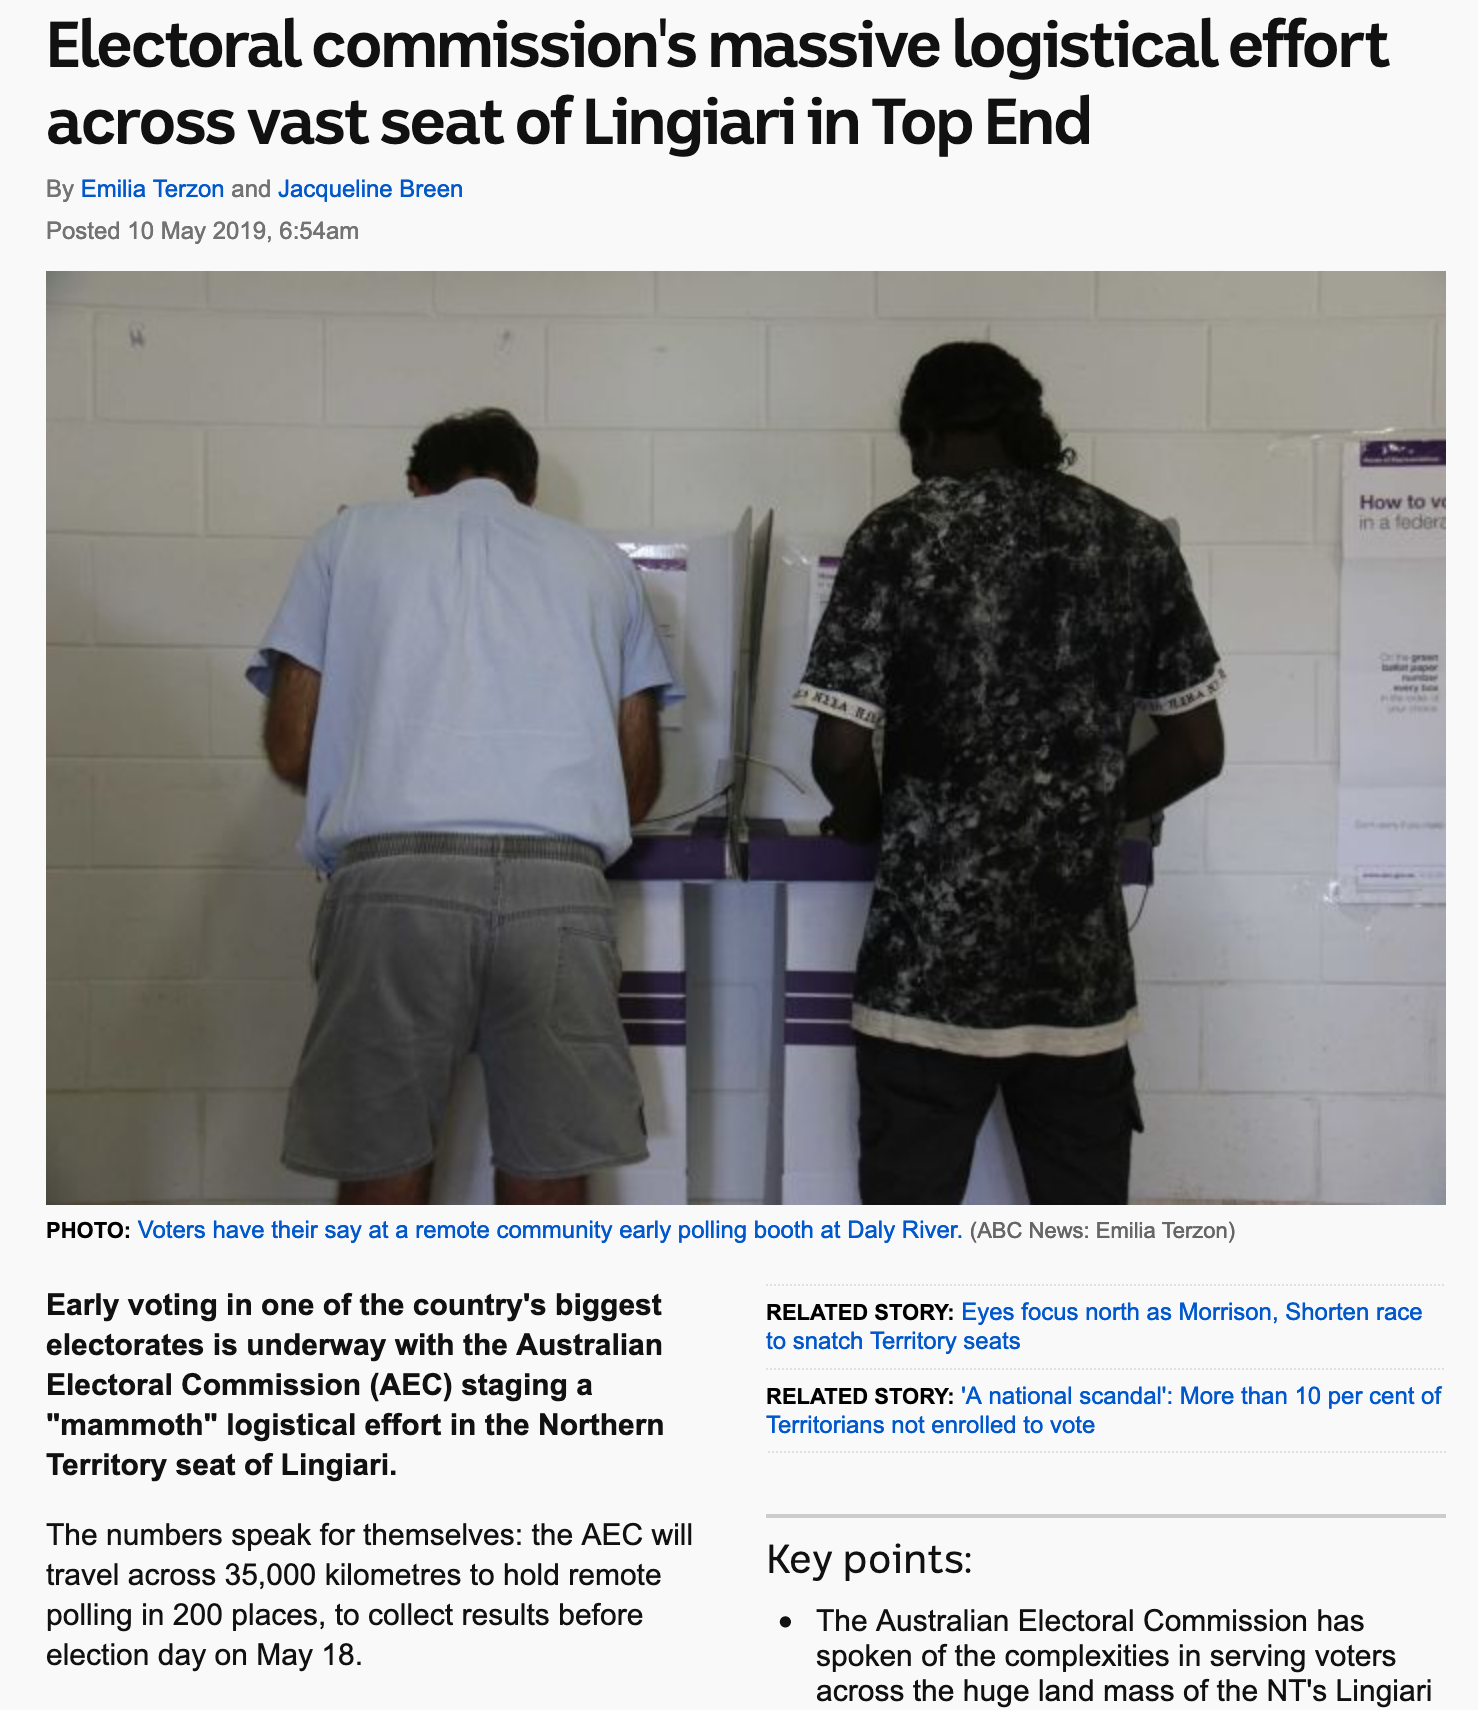
\includegraphics[scale=0.20]{logistic.png}
	\end{center}
  \end{figure} 
\end{frame}


%
%\begin{frame}
%\frametitle{Background}
%{Everything works great with paper ballot except}
%\begin{itemize}
%\item Slow for big countries like India
%\item Counting is error prone for complex method like STV
%\item Logistic challenge for sparsely populated countries Australia 
%\end{itemize}
%\end{frame}

\begin{frame}
\frametitle{Electronic Voting}
{Enter the realm of Electronic Voting}
\begin{figure}
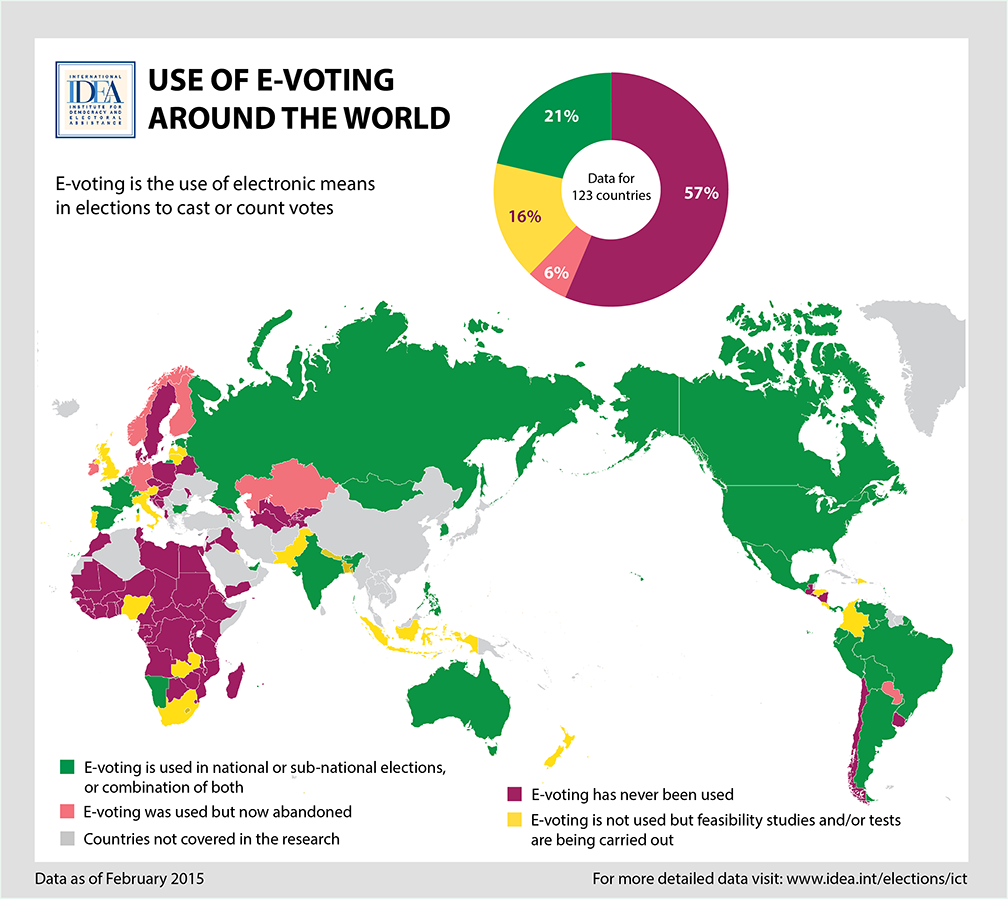
\includegraphics[scale=0.20]{e-voting-map.png}
\end{figure}
\end{frame}


\begin{frame}
\frametitle{Electronic Voting}
{Could not configure the proper SSL certificates: FREAK Attack}
\begin{figure}
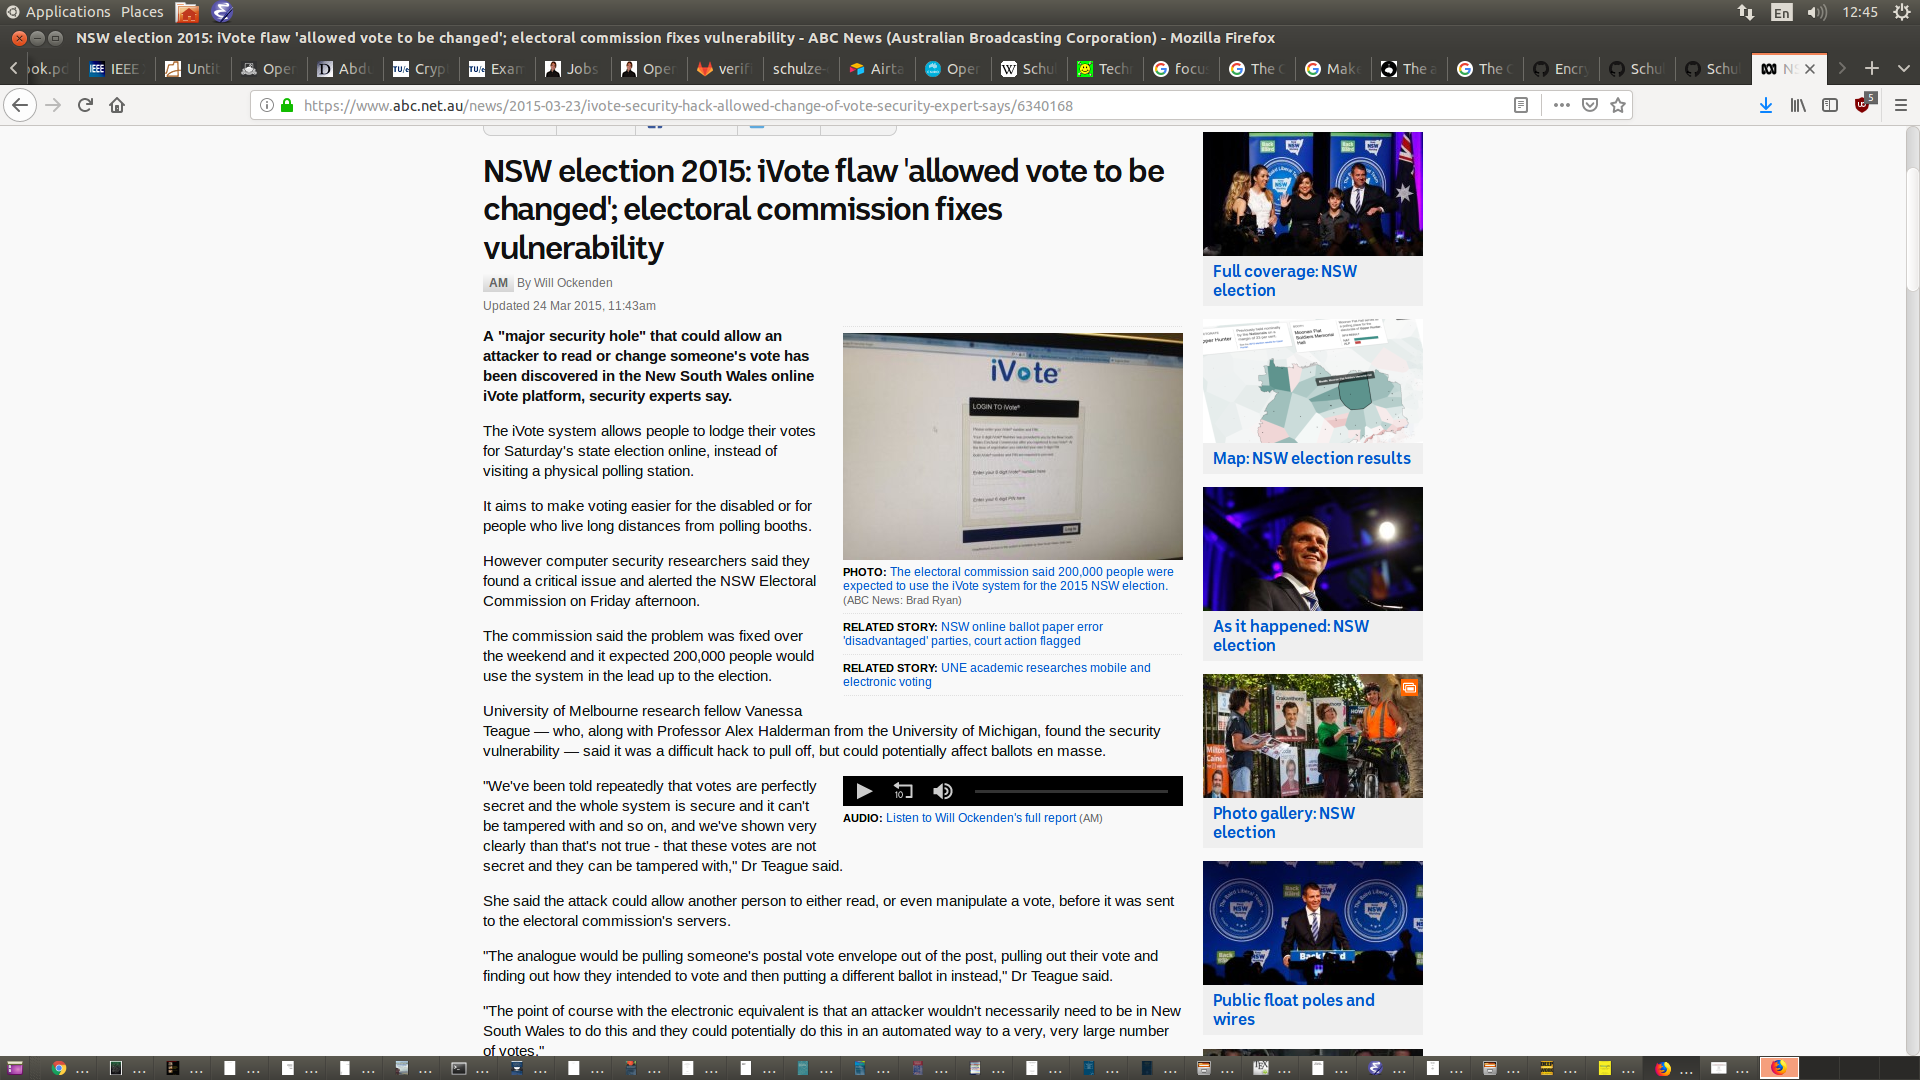
\includegraphics[scale=0.20]{Ausvoting.png}
\end{figure}
\end{frame}



\begin{frame}
\frametitle{Electronic Voting}
{Security by obscurity: Easy to manipulate ballots by using a mobile phone}
\begin{figure}
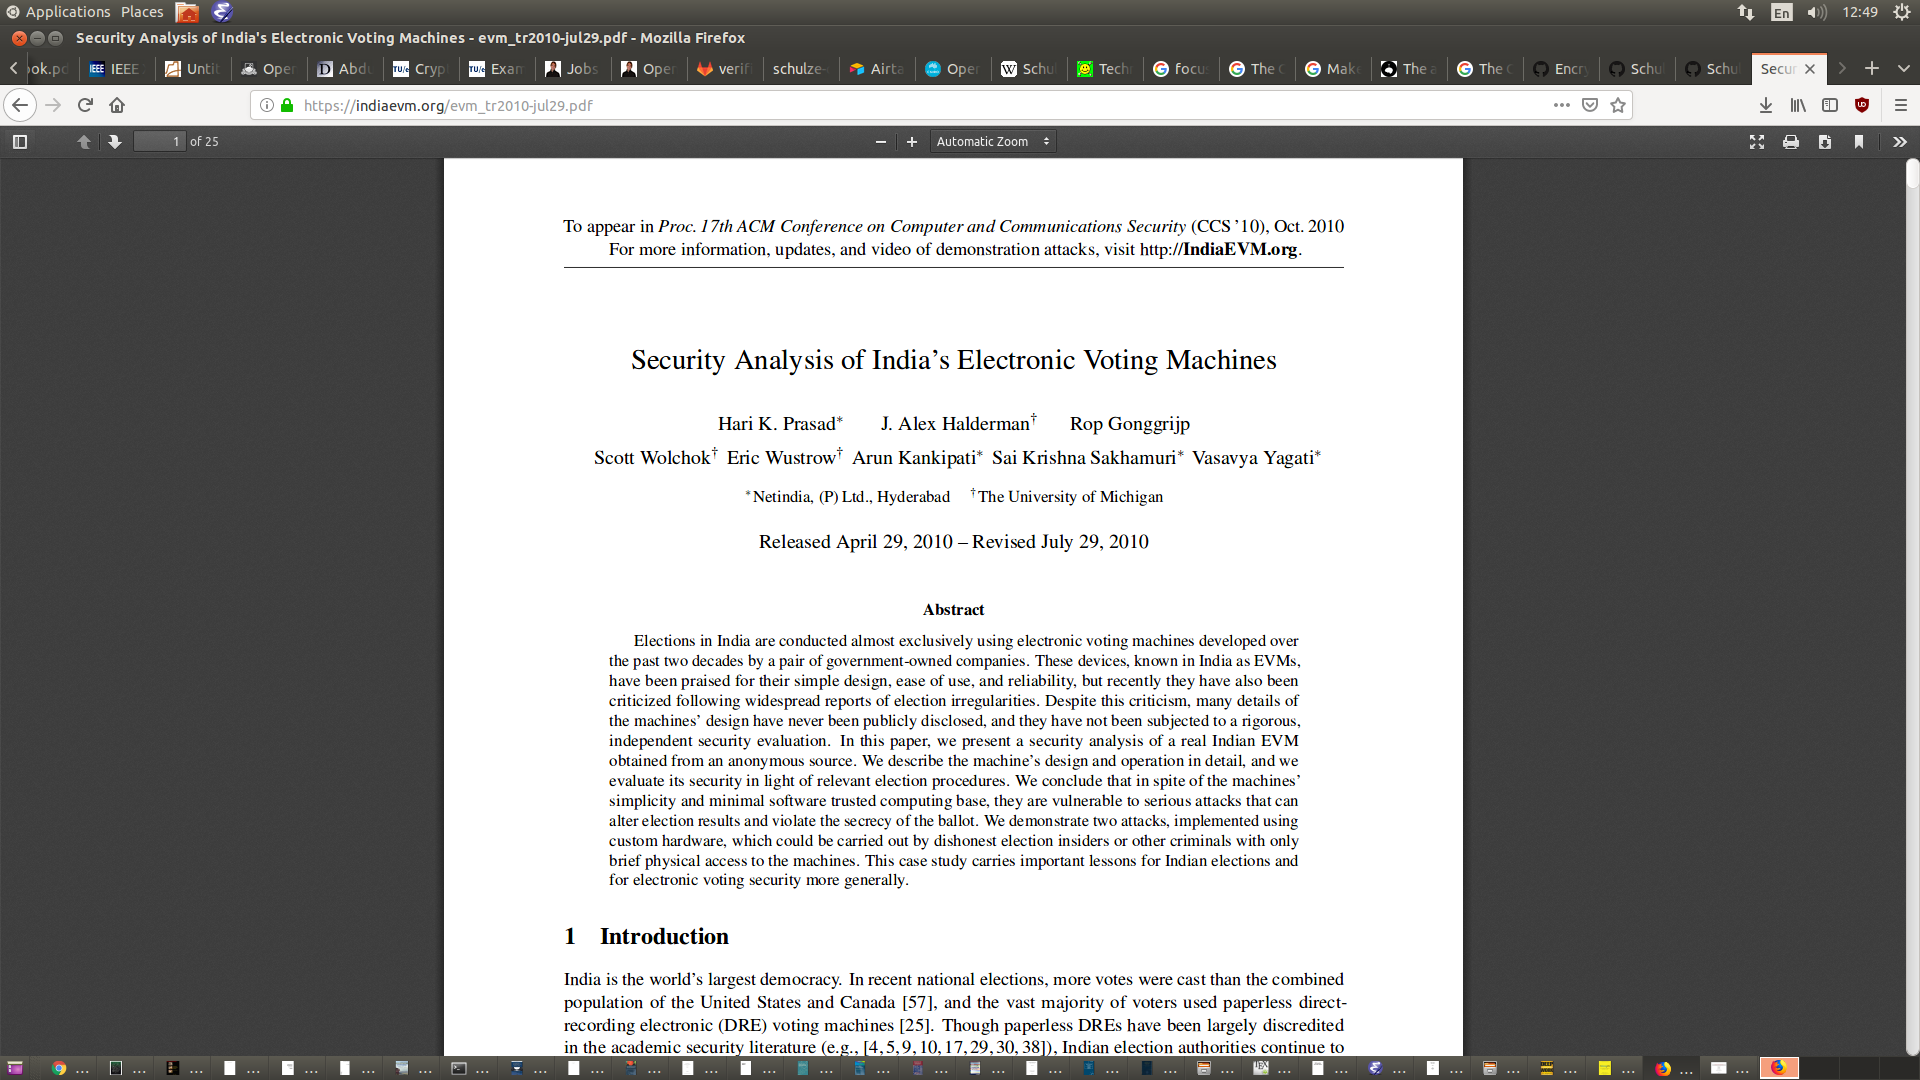
\includegraphics[scale=0.20]{Indiavote.png}
\end{figure}
\end{frame}


\begin{frame}
\frametitle{Electronic Voting}
{Parameter generation}
\begin{figure}
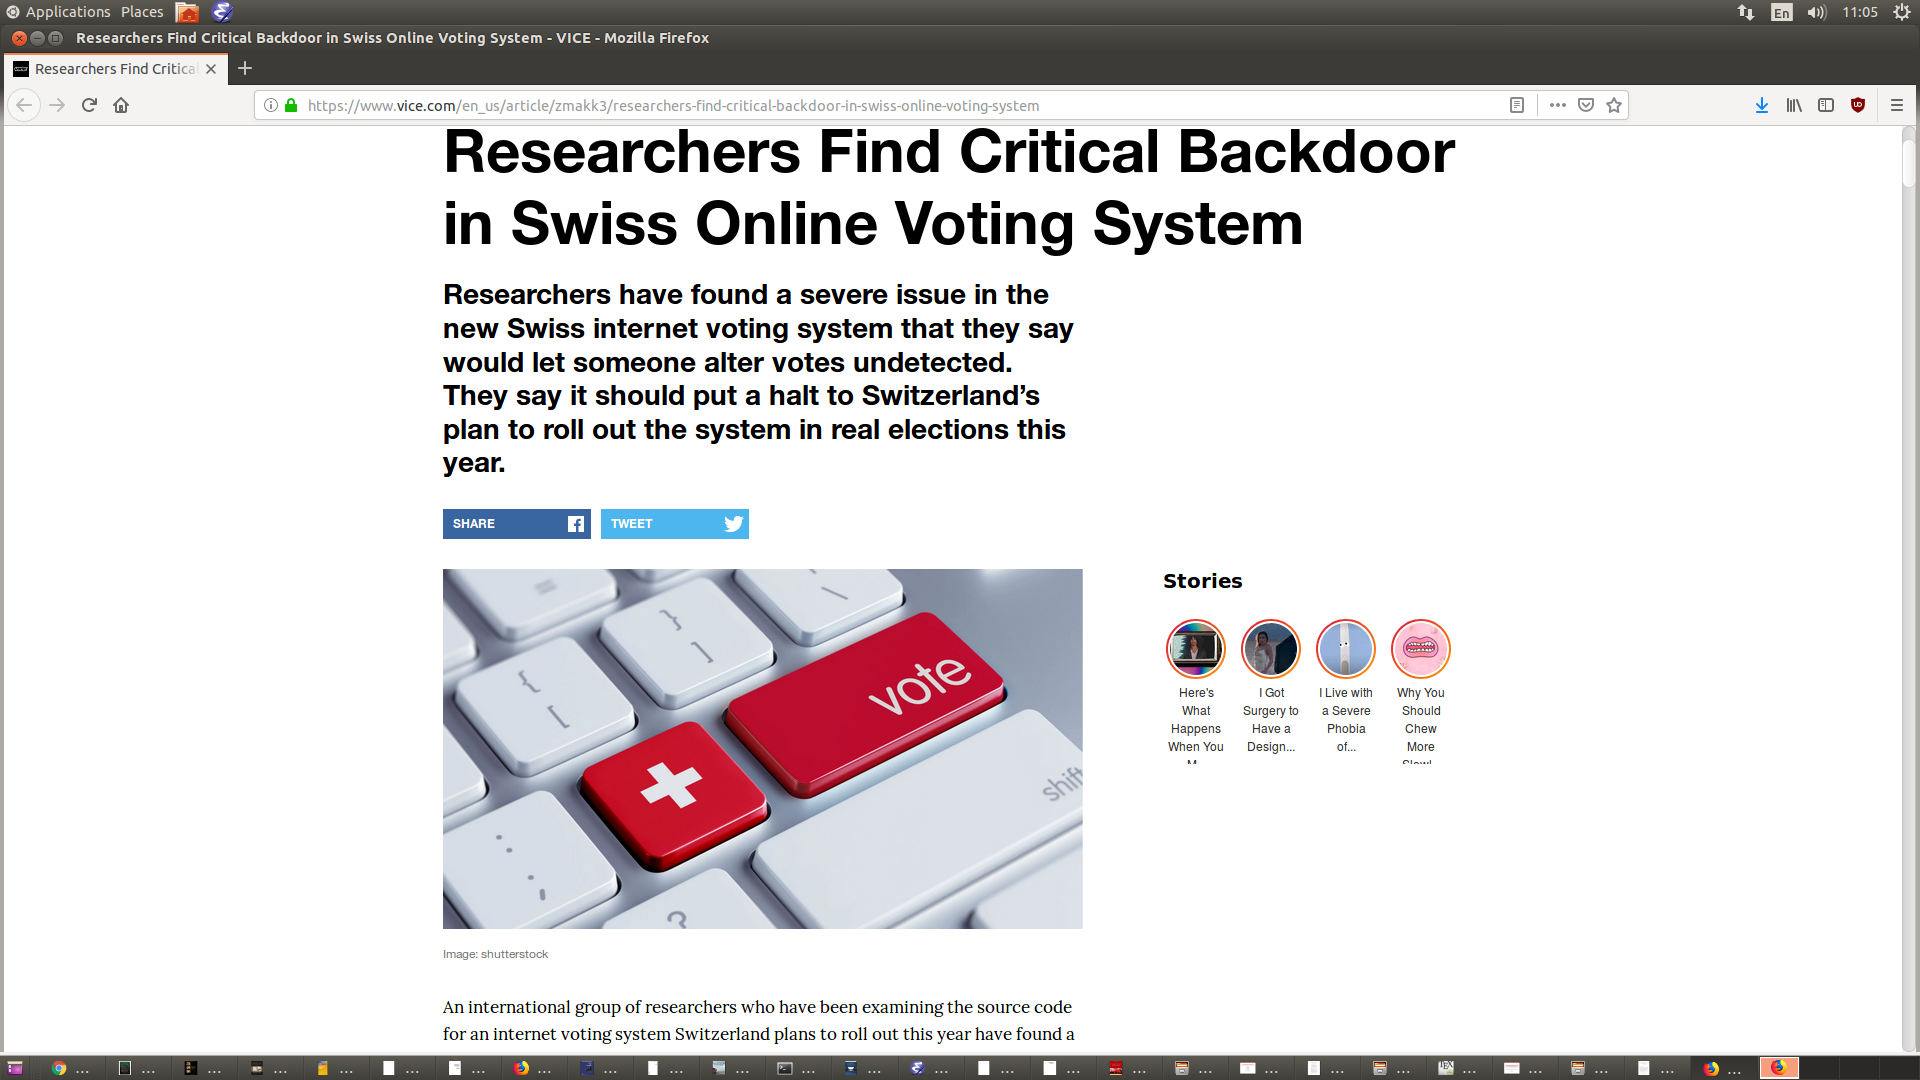
\includegraphics[scale=0.20]{swisspost.png}
\end{figure}
\end{frame}




\begin{frame}
\frametitle{Motivation}
{Could not count properly}
\begin{center}
\begin{tikzpicture}
  \node (img1) {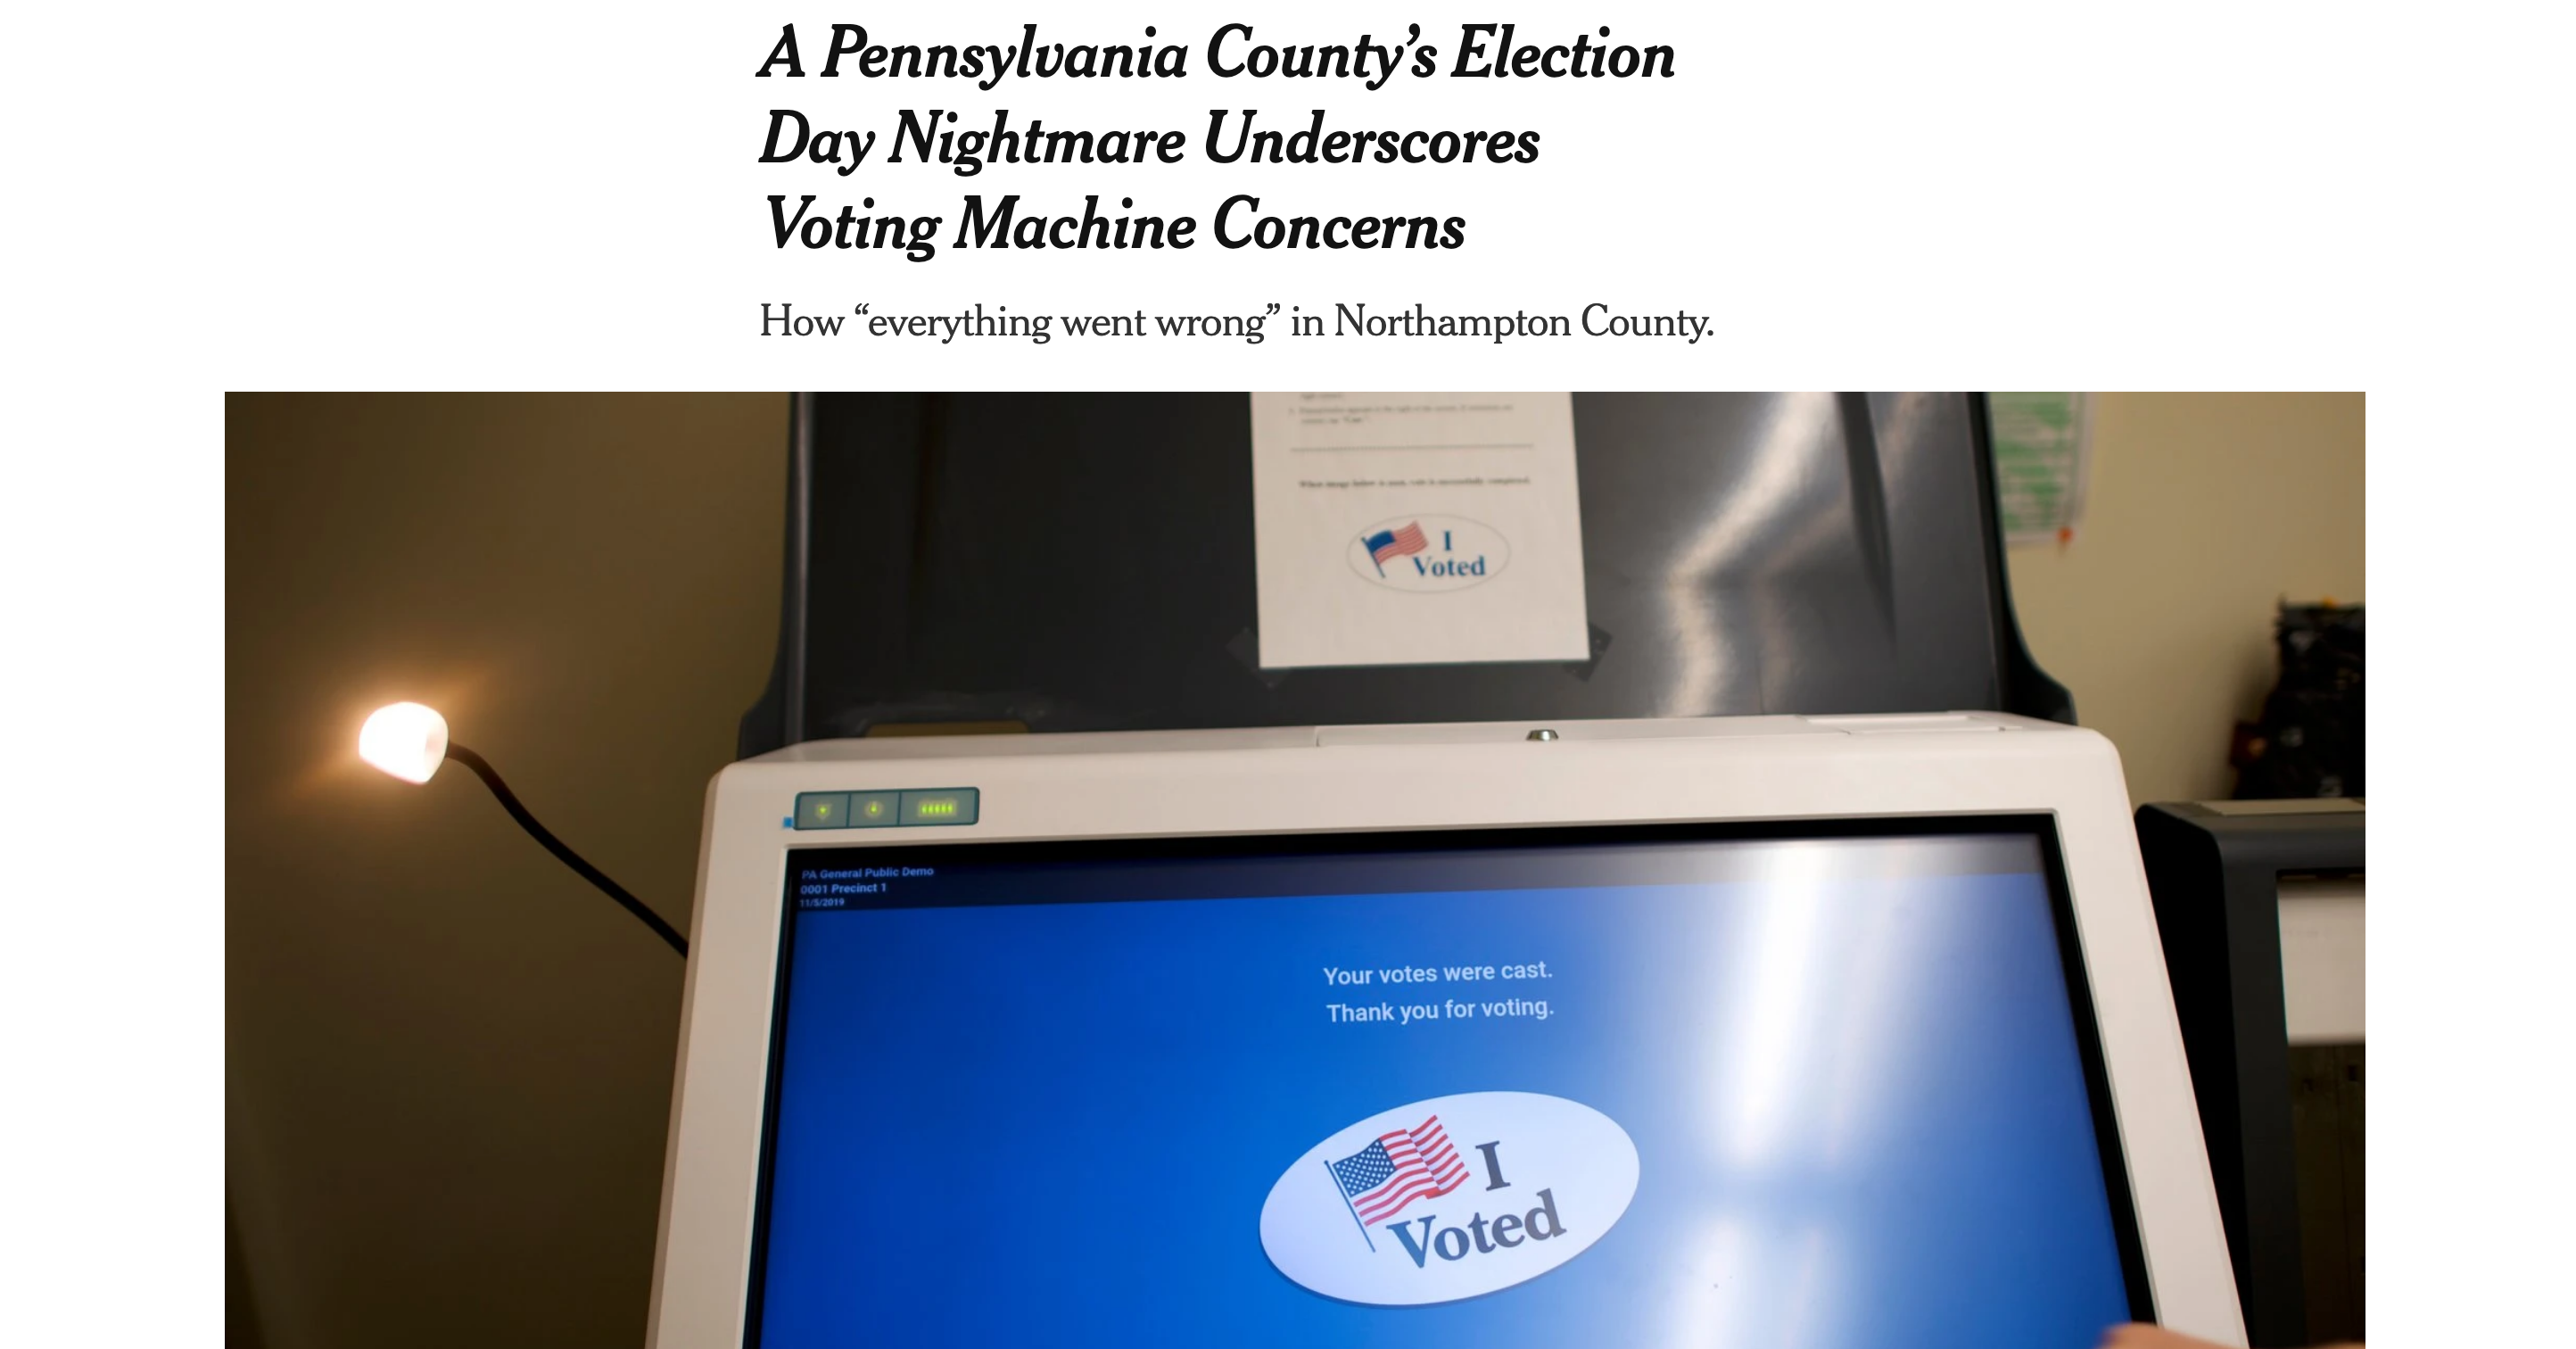
\includegraphics[height=4cm]{counting-bug.png}};
  \pause
  \node (img2) at (img1.south east) {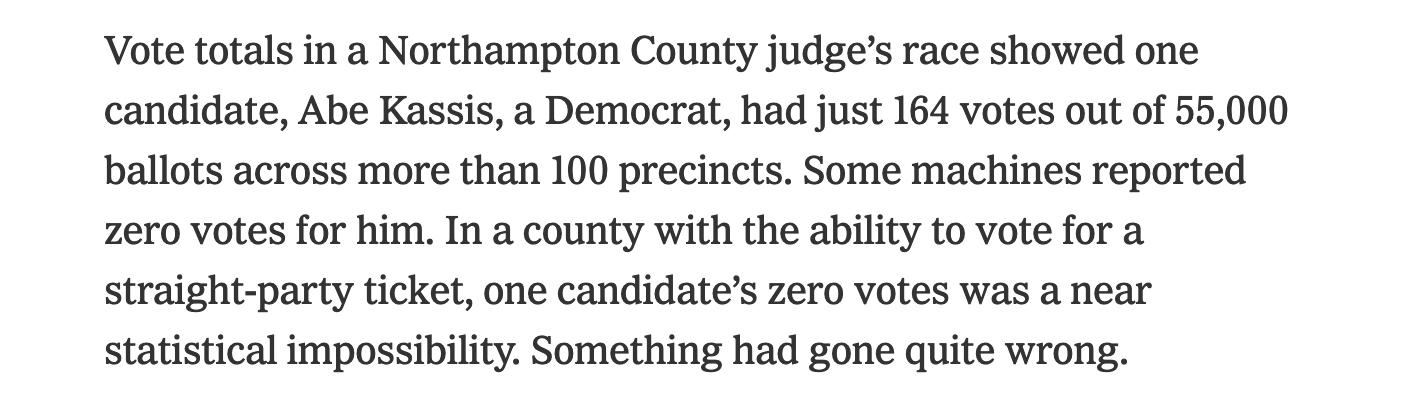
\includegraphics[height=2cm]{explanation.png}};
\end{tikzpicture}
\end{center}
\end{frame}


%\begin{frame}
%\frametitle{Motivation}
%\begin{figure}
%	\begin{center}
%	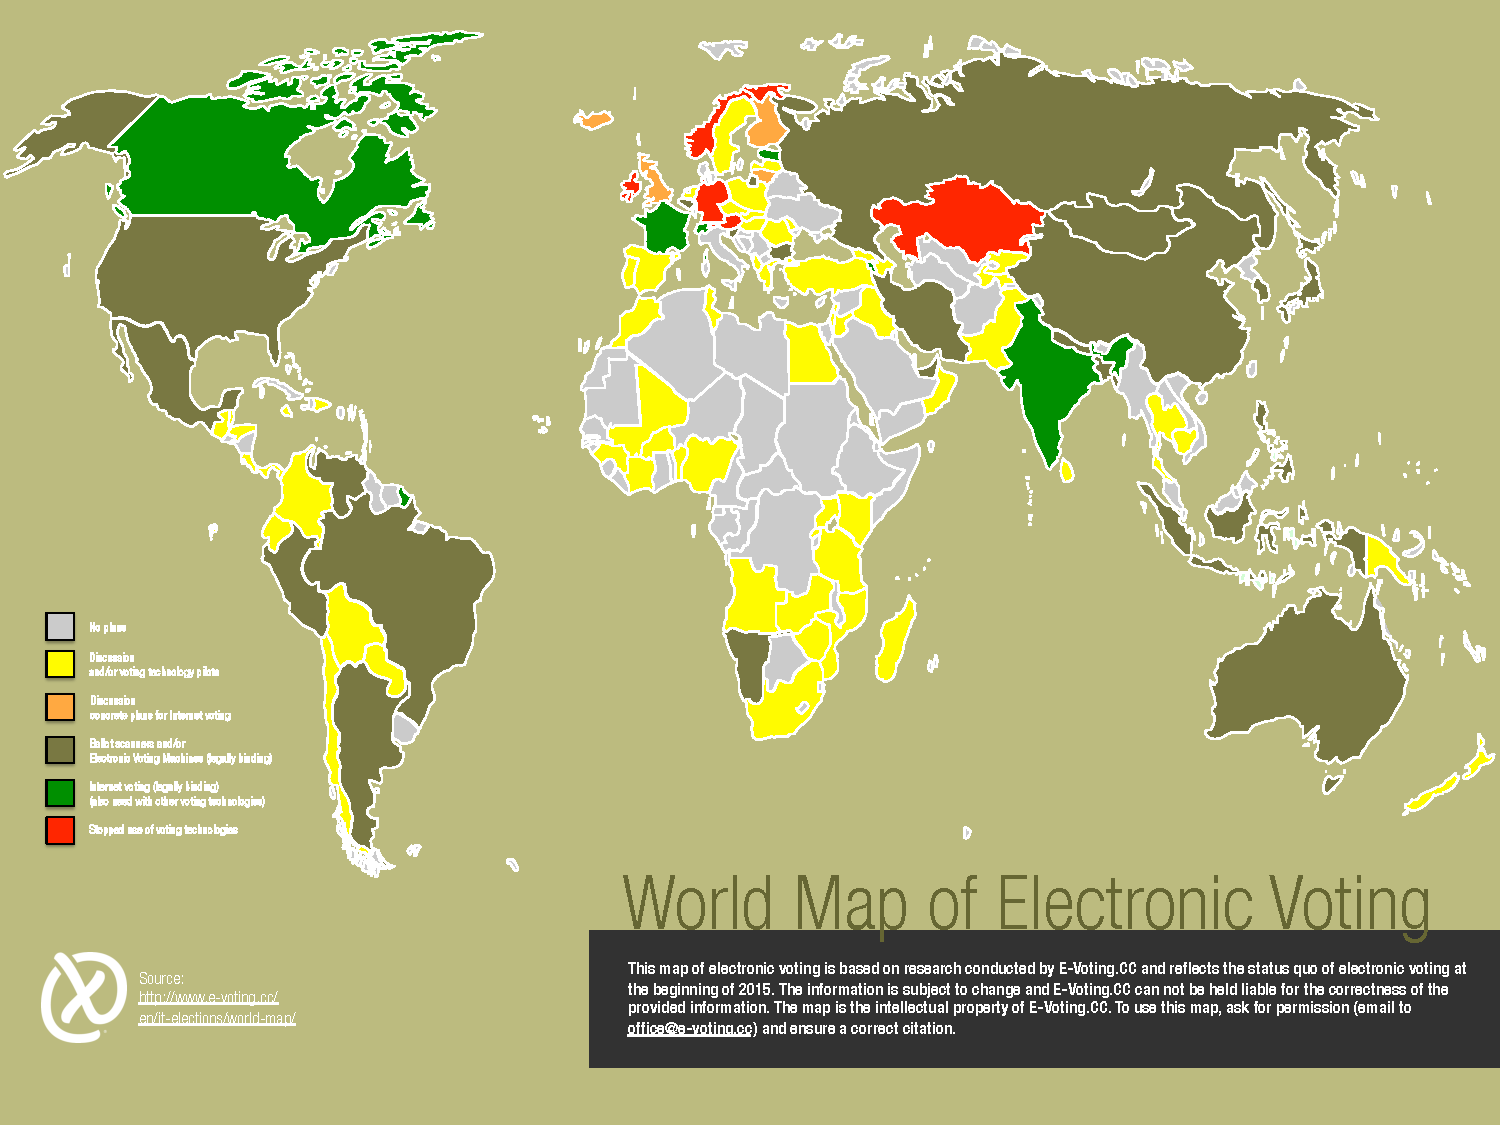
\includegraphics[scale=0.30]{e-voting_worldmap_2015.pdf}
%	\end{center}
%  \end{figure}
%\end{frame}


\begin{frame}
\frametitle{Electronic Voting}
{Countries in the Pink}
\begin{figure}
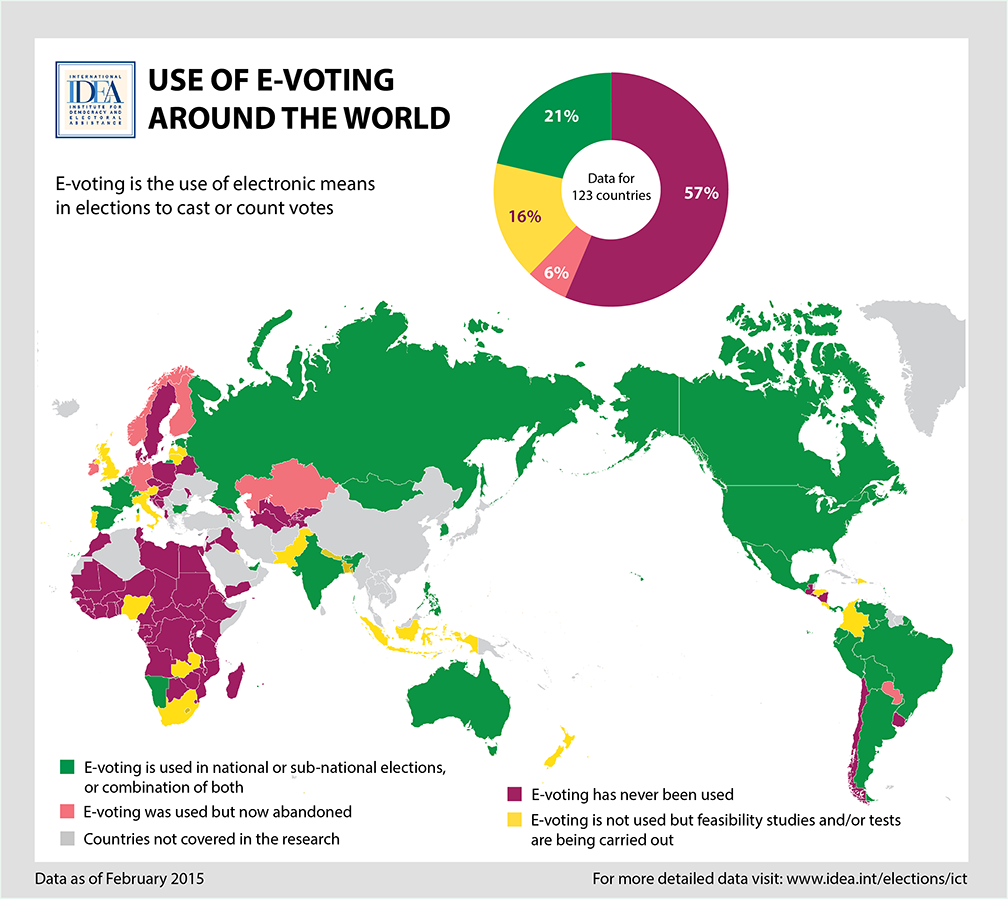
\includegraphics[scale=0.20]{e-voting-map.png}
\end{figure}
\end{frame}

\begin{frame}
\frametitle{Withdrawn from Electronic Voting}
\begin{itemize}
\item Netherlands: Information Leakage
\item Germany: Not Verifiable
\end{itemize}
\end{frame}


\begin{frame}
\frametitle{Take Away: Very difficult to achieve in Electronic Setting}
\begin{itemize}
\item Correctness
\item Verifiability
\item Privacy
\end{itemize}
\end{frame}



\begin{frame}
\frametitle{Correctness by }
\begin{center}
\begin{tikzpicture}
  \node (img1) {
\includegraphics[height=6cm]{coq.png}};
%  \pause
%  \node (img2) at (img1.south east) {
\includegraphics[height=6cm]{coq.png}};
\end{tikzpicture}
\end{center}
\end{frame}

\begin{frame}
\frametitle{Coq in Action}
{Natural Number with addition function and proof of 
commutativity and associativity}
\lsteighteen
\end{frame}


\begin{frame}
\frametitle{Coq in Action}
{Graph Theory}
\lstf
\end{frame}

\begin{frame}
\frametitle{Definition and Assumption}
\begin{itemize}
\item End to End verifiability
\begin{itemize}
  \item<.-> every voter can verify that their ballot was cast as
  intended
  \item every voter can verify that their ballot was collected as
  cast
  \item everyone can verify final result on the basis of the
  collected ballots.
\end{itemize}

%\item We are not concern with any front end activity
\item We assume first two part of \textit{End to End verifiability} and work on
      third part.
\end{itemize}
\end{frame}



\begin{frame}
\frametitle{Verifiability by Scrutiny Sheet}
\lstnineth
\end{frame}


\begin{frame}
\frametitle{Privacy by Homomorphic Encryption}
\begin{itemize}
\item A encryption scheme is homomorphic if for any two plaintext $x$ and $y$:
$Enc_{pk}(x) \bigotimes Enc_{pk}(y) = Enc_{pk} (x \bigoplus y)$
\item $Enc(m_{1}, r_{1}) := (g^{r_{1}}, g^{m_{1}} *  h^{r_{1}})$ 
\item $Enc(m_{2}, r_{2}) := (g^{r_{2}}, g^{m_{2}} *  h^{r_{2}})$
\item  $Enc(m_{1}, r_{1})  * Enc(m_{2}, r_{2}) $ =  ($g^{r_{1} + r_{2}}$, $g^{m_{1} + m_{2}} * h^{r_{1} + r_{2}}$) 		
		
\end{itemize}
\end{frame}

\begin{frame}
\frametitle{In Reality, it looks more messy}
$g = 4, h = 49228593607874990954666071614777776087$
 (134496451437300221012286033361707130093, 102227210111257780065764179227658264107)
 
 (90549562016409048906553052880573051723, 149737664809130232173423485580305447580)
  
 (111838646913099268144525651231935275385, 23076766166773179621624801755228562722) 
 
 (163609675266885117507253145530469574507, 136840925491933116006881481565552266698)
% (79248907920406812537389036699896088139, 46347343081571464310476936648567024138)
% (123866687819159436288533311854341351671, 147511135596830390870297120177829059519)
% (50398592318313244808461064689068665943, 53262724480261770219974712577122611417)
% (7017345267197193636466005866496039911, 68311911432471947228868781091036768394)
% (23649424831721765685116725354379513587, 82314118594242117678180792762644770882)
\end{frame}



\begin{frame}
\frametitle{Zero-Knowledge-Proof}
{Did you all trust me when I claimed that the all the values are encryption of 0?}
\begin{figure}

\includegraphics[scale=0.30]{pilot.png}
\end{figure}

\end{frame}


\begin{frame}
\frametitle{Zero-Knowledge-Proof}
\begin{itemize}
\item Given a public parameters $(G, g, p, h)$ and private parameter $x$ such that $h := g^x$.
\item Claim: message $m$  is honest decryption of $(c_{1}, c_{2})$ (where $c_{1} = g^r$ and $c_{2} = g^{m} * h^{r}$)
\item Proof: $(g, h, c_{1}, c_{2} \cdot g^{-m})$ is a \textit{Diffie Hellman} tuple 
\end{itemize}
\end{frame}


\begin{frame}
\frametitle{Zero-Knowledge-Proof}
\textbf{Diffie Hellman Tuple:} a tuple $(g, h, u, v)$ is 
 a \textit{Diffie Hellman} tuple if there $\exists$ $w \mid$
 $u = g^w \land v = h^w$. 
 
 \begin{itemize}
 \item $P$ chooses a random $r$ and sends $a=g^r$ and $b = h^r$.
 \item $V$ sends a random $e$
 \item $P$ sends $z =r + e \cdot w$
 \item $V$ check $g^z = a \cdot u^e$ and $h^z = b\cdot v^e$ 
 \end{itemize}
 $g^z = g^{r + e \cdot w} = a \cdot (g^w)^e = a \cdot u^e $\\
 $h^z = h^{r + e \cdot w} = b \cdot (h^w)^e = b \cdot v^e$
\end{frame}

\begin{frame}
\frametitle{Zero-Knowledge-Proof}
{Claimed: $(g, h, c_{1}, c_{2} \cdot g^{-m})$ is a \textit{Diffie Hellman} tuple}
$(g, h, c_{1}, c_{2} \cdot g^{-m})$\\
$ = (g, h, g^r, g^m \cdot h^r \cdot g^{-m})$ \\
$ = (g, h, g^r, h^r)$ \\
$ = (g, h, u, v)$\\ 
{Could I have faked it?} \\
$(g, h, g^r, g^m \cdot h^r \cdot g^{-m_{1}})$ \\
$ = (g, h, g^r, h^r \cdot g^{m - m_{1}})$

\end{frame}


\begin{frame}
\frametitle{Schulze Voting as Evidence Carrying Computation}
\begin{itemize}[]
\item Pros 
\begin{itemize}
\item Formally verified implementation in Coq
\item Verifiable because we generate certificate
\item Certificates are accessible to anyone with 
      basic math literacy
\end{itemize}
\item Cons
\begin{itemize}
\item Horribly slow and not practical for real life election
\item No privacy and possibly susceptible to coercion
\end{itemize}
\end{itemize}
\end{frame}


\begin{frame}
\frametitle{Scaling it to count millions ballot }
\begin{itemize}[]
\item Pros 
\begin{itemize}
\item Formally verified implementation in Coq
\item Verifiable because we generate certificate
\item Certificates are accessible to anyone with 
      basic math literacy
\item Blazing fast for real life elections
\end{itemize}
\item Cons
\begin{itemize}
\item No privacy and possibly susceptible to coercion
\end{itemize}
\end{itemize}
\end{frame}



\begin{frame}
\frametitle{Verifiable Homomorphic Tallying for the Schulze Vote Counting Scheme}
\begin{itemize}[]
\item Pros 
\begin{itemize}
\item Formally verified implementation in Coq assuming axioms on 
          the cryptographic primitives 
\item Verifiable because we generate certificate 
\item Privacy because we don't reveal the content of ballots
\end{itemize}
\item Cons
\begin{itemize}
\item Horribly Slow (10,000 ballots in 25 hours)
\item Certificates are only accessible to someone having specialized 
	  knowledge of cryptography
\item Trusting on Java code in realized extracted code
\end{itemize}
\end{itemize}
\end{frame}


\begin{frame}
\frametitle{Certificate : Verifying Elections Formally}
\begin{itemize}
\item We developed a general framework for Sigma Protocol
\item Instantiate with IACR 2018 election data
\item We proved some computationally intense result inside 
      Coq
\end{itemize}
\end{frame}



\begin{frame}
\frametitle{Machine Check Properties}
\begin{itemize}
\item Condercet Winner (Finished)
\item Reversal symmetry (Finished)
\item Monotonicity
\item Smith Set
\end{itemize}
\end{frame}

\begin{frame}
\frametitle{Future Work}
\begin{itemize}
\item Formalizing cryptographic code (Shuffle Proof)
\item Formalizing the properties of Schulze method
\item Formaly verified checker 
\item Risk Limiting Audit 
\item Formalizing Code Extraction (Not related to our project, but highly needed for electronic voting)
\end{itemize}
\end{frame}

\begin{frame}
\frametitle{Publications}
\begin{enumerate}
	\item Pattinson, D. and Tiwari, M., 2017. Schulze Voting as Evidence carrying computation. In Proc. 
	ITP 2017, vol. 10499 of Lecture Notes in Computer Science, 410–426. Springer. 
	\item Lyria Bennett Moses, Rajeev Goré, Ron Levy, Dirk Pattinson, Mukesh Tiwari.
	No More Excuses: Automated Synthesis of Practical and Verifiable Vote-Counting Programs for Complex 
	Voting 	Schemes. E-VOTE-ID 2017: 66-83
	\item Thomas Haines, Dirk Pattinson, and Mukesh Tiwari. 2019. 
	  Verifiable Homomorphic Tallying for the Schulze Vote Counting Scheme. 
	  11th International Conference Verified Software: Theories, Tools, and Experiments. 
      VSTTE 2019 (to appear)	
	\end{enumerate}
\end{frame}

\begin{frame}
\frametitle{Publications}
\begin{enumerate}
	 
	\item Thomas Haines, Rajeev Goré, and Mukesh Tiwari. 2019. Verified Verifiers for Verifying Elections. 
	 In Proceedings of the 2019 ACM SIGSAC Conference on Computer and Communications Security (CCS '19)
	 
	 \item Milad K. Ghale, Rajeev Goré, Dirk Pattinson, Mukesh Tiwari.
	Modular Formalisation and Verification of STV Algorithms. E-Vote-ID 2018: 51-66
	\end{enumerate}
\end{frame}
%
%
%\begin{frame}
%\frametitle{Why Schulze Method ?}
%\begin{itemize}
%\item Although Schulze method is not used in any parliamentary elections, but it's 
%      de facto standard in many communities over Internet. It is used 
%	 used in the elections of almost 60 organization including Free Software Foundation, Gentoo Foundataion, Haskell and Pirate Party of many countries. Part of the reason for its popularity is that no preferential voting scheme can guarantee
%all desirable properties that one would like to impose due to Arrow’s theorem [2], the Schulze method offers a good compromise, with a number of important properties
%already  established  in  Schulze’s  original  paper, like monotonicity, Condorcet consistency, and Majority.
%
%
%%\item Gaining popularity in the open source community\pause
%%\item Quantative comparison by Rivest and Shen
%%\item Lots of good properties e.g. monotonicity, majority, condercet\pause 
%%\item Trust in electronic elections using formal verification [ITP 2017]\pause
%%\item Case study to demonstrate real world counting [E-Vote-ID 2017]
%\end{itemize}
%\end{frame}


%\begin{frame}
%\frametitle{Schulze Method}
%\begin{itemize}
%\item Collective preferences can be cyclic, even if the preferences of individual voters are not cyclic.
%\end{itemize}
%\begin{figure}[ht]
%\centering
%$
%\xymatrix@R=12ex@C=12ex{
%A \ar@/^/[rr]^{3} \ar@/_/[dr]_{-1} & & B \ar@/^/[ll]^{-3}
%\ar@/^/[dl]^5 \\
%& C \ar@/_/[ul]_{1} \ar@/^/[ur]^{-5}
%}$\end{figure}
%\begin{itemize}
%\item The main idea of the method is to resolve cycles by considering \emph{transitive preferences} or a generalised notion of margin.
%\end{itemize}
%\end{frame}

%\begin{frame}
%\frametitle{Schulze Method}
%
%\begin{itemize}
%\item Consider an election with a set of $m$ candidates $C$ = $\{c1,\dots,cm\}$, and 
%	a set of $n$ votes $P$ = $\{b1,\dots,bn\}$. A vote
%	is represented as function $b: C \rightarrow \mathbb{N}$ that assigns natural 
%	number (the preference) to each candidate, and we recover a strict linear  
%	preorder $<_b$ on candidates by setting $c <_b d$ if $b(c) > b(d)$.
%
%	%\begin{wrapfigure}[14]{r}[0cm]{0.4\textwidth}
%  %\begin{center}
%    %\raisebox{0pt}[-1cm]
%    \raisebox{0pt}[\dimexpr\height-0.5\baselineskip\relax]
%    {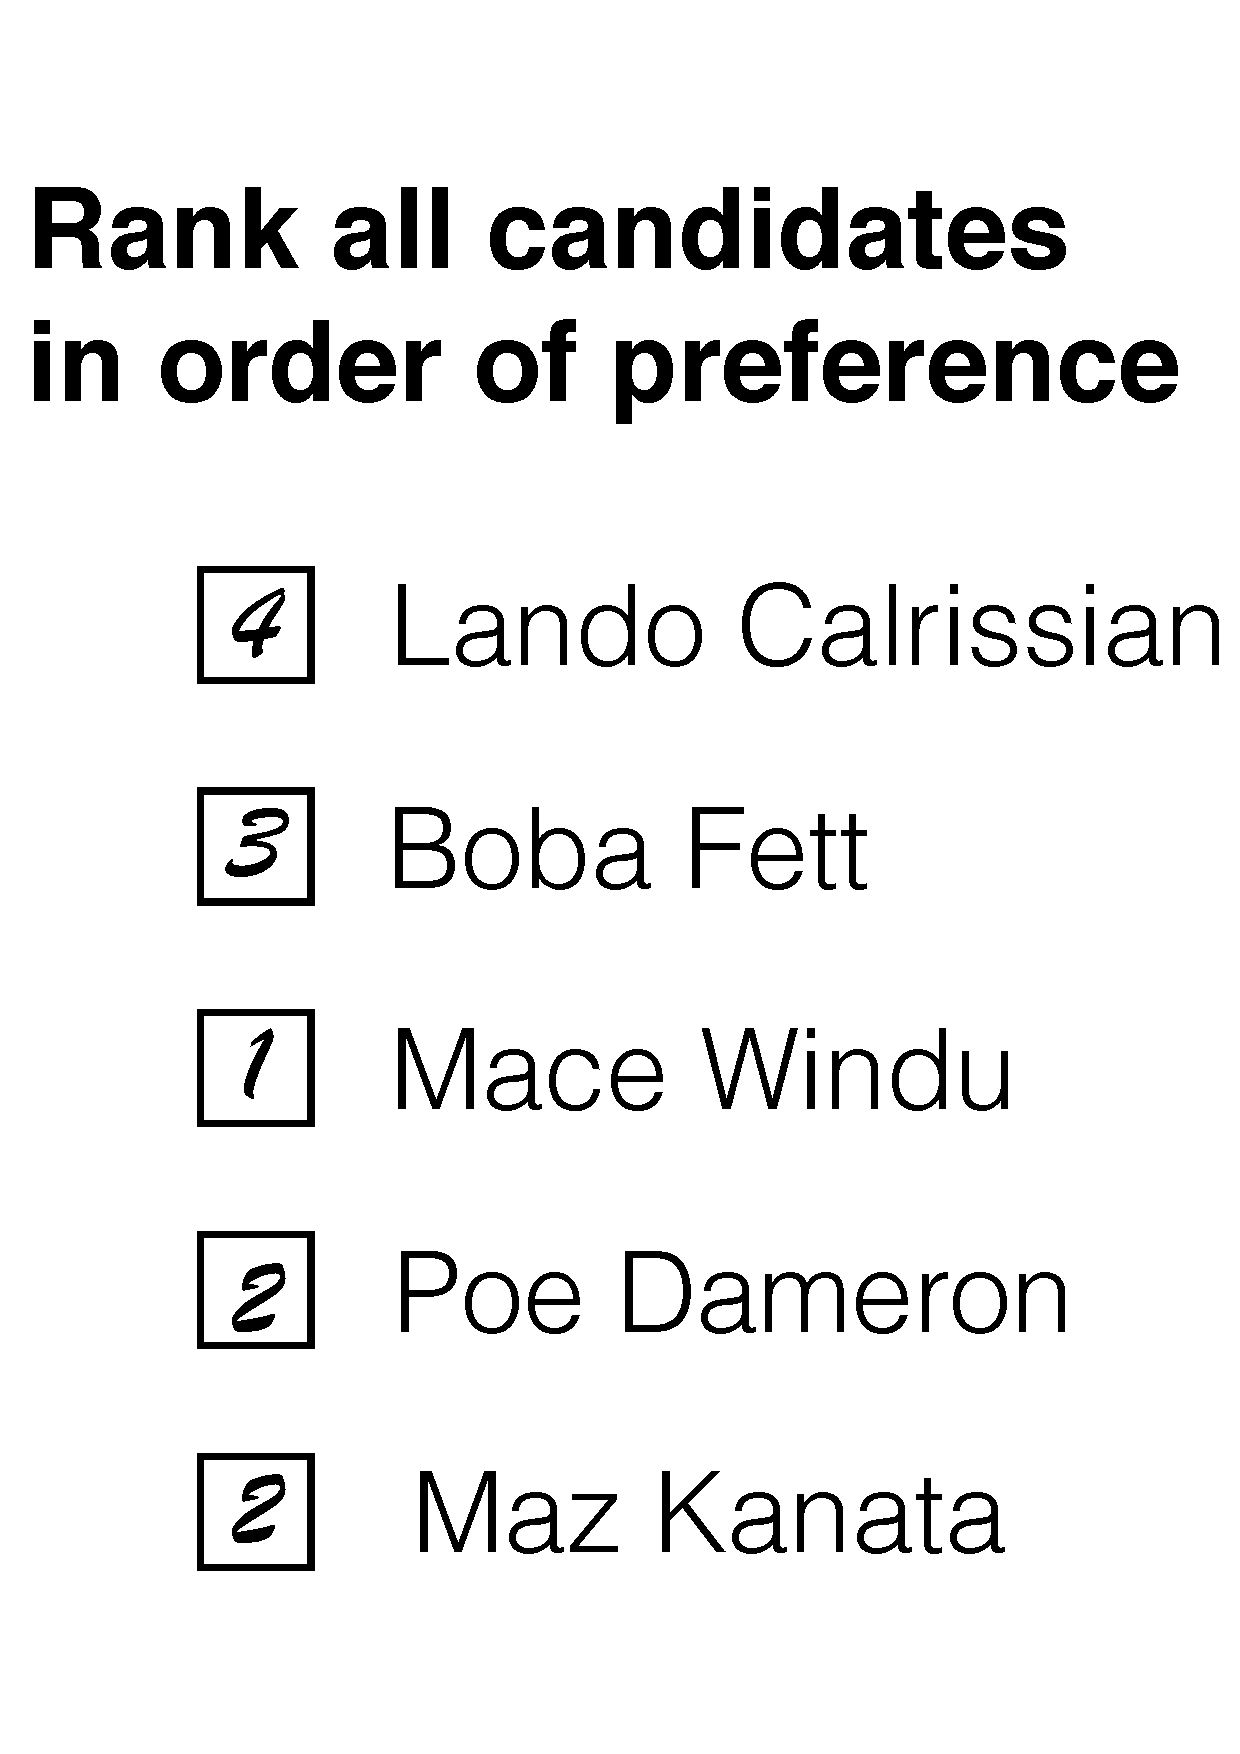
\includegraphics[width=0.37\textwidth]{bal-cropped.pdf}}
%    \raisebox{0pt}[\dimexpr\height-8.5\baselineskip\relax]{xx}
%    %\includegraphics[width=4cm]{ballot.png}
%  %\end{center}
%  %\end{wrapfigure}







%\item The \emph{margin function} $m(c, d)$ as the number of
%ballots that strictly prefer $c$ over $d$, minus the number of
%ballots that strictly prefer $d$ over $c$\pause
%\item Schulze voting considers \emph{paths} of the form \[\xymatrix@C=10ex{ c_1  \ar[r]^{m(c_1, c_2)} & c_2   \ar[r]^{m(c_2,c_3)} & c_3 \ar@{}[r]|{\dots} & c_{n-1}   \ar[r]^{m(c_{n-1}, c_n)} & c_n } \]\pause
%\item  Path-based margin  between $c_1$ and $c_n$ is $\min \lbrace m(c_i, c_{i+1} \mid 1 \leq i < n \rbrace$\pause 
%\item The \emph{generalised margin} between two candidates $c$ and $d$ is the largest path-based margin considering all possible paths between $c$ and $d$.
%
%\end{itemize}
%\end{frame}

%
%\begin{frame}
%\frametitle{Schulze Method}
%\begin{itemize}
%
%\item Given a set of ballots $P$ and candidate set $C$, we construct graph $G$ based on the margin function $m: C \times C \to \mathbb{Z}$. Given two candidates $c, d \in C$,
%the \emph{margin} of $c$ over $d$ is
%the number of voters that prefer $c$ over $d$, minus the number of voters that prefer $d$ over $c$. In symbols
%\[
%  m(c, d) = \sharp \lbrace b \in P \mid c >_b d \rbrace -
%            \sharp \lbrace b \in P \mid d >_b c \rbrace
%\] where $\sharp$ denotes cardinality and $>_b$ is the strict
%(preference) ordering given by the ballot $b \in P$.
%\end{itemize}
%\end{frame}
%
%\begin{frame}
%\frametitle{Schulze Method}
%\begin{itemize}
%\item Example of Graph G (collective preferences can be cyclic, even if the preferences of individual voters are not cyclic). The main idea of the method is to resolve cycles by considering \emph{transitive preferences} or a generalised notion of margin.
%\[
%\xymatrix@R=12ex@C=12ex{
%A \ar@/^/[rr]^{3} \ar@/_/[dr]_{-1} & & B \ar@/^/[ll]^{-3}
%\ar@/^/[dl]^5 \\
%& C \ar@/_/[ul]_{1} \ar@/^/[ur]^{-5}
%}\]
%\end{itemize}
%\end{frame}
%
%
%\begin{frame}
%\frametitle{Schulze Method}
%\begin{itemize}
%
%\item A directed \emph{path} in graph, $G$, from
%candidate $c$ to candidate $d$ is a sequence $p \equiv c_0, \dots, c_{n+1}$
%of candidates with $c_0 = c$ and $c_{n+1} = d$ ($n \geq 0$), and the
%\emph{strength}, st, of path, p, is the minimum margin of adjacent
%nodes, i.e.
%\[ st(c_0, \dots, c_{n+1}) = \min \lbrace m (c_i, c_{i+1}) \mid 0
%\leq i \leq n \rbrace. \]
%\item For candidates c and d, let $S(c, d)$ denote the maximum strength, or generalized margin of a path
%	from c to d i.e. 
%	\[ S(c, d) = \max \lbrace st (p) : \text{p is path from c to d in G} \rbrace\]
%	
%\item The winning set (always non empty) is defined as 
% \[ W =  \lbrace c \in C : \forall d \in C \setminus \{c\}, S (c, d) \geq S (d, c) \rbrace\]
%
%\end{itemize}
%\end{frame}


%
%\begin{frame}
%\frametitle{Example of Schulze method}
%\[
%\xymatrix@R=12ex@C=12ex{
%A \ar@/^/[rr]^{3} \ar@/_/[dr]_{-1} & & B \ar@/^/[ll]^{-3}
%\ar@/^/[dl]^5 \\
%& C \ar@/_/[ul]_{1} \ar@/^/[ur]^{-5}
%} \qquad \xymatrix@R=12ex@C=12ex{
%A \ar@/^/[rr]^{3} \ar@/_/[dr]_{3} & & B \ar@/^/[ll]^{1}
%\ar@/^/[dl]^5 \\
%& C \ar@/_/[ul]_{1} \ar@/^/[ur]^{1}
%}\]
%\end{frame}
%
%
%
%
%\begin{frame}
%\frametitle{Coq formalization}
%\begin{itemize}
%\item To demonstrate that a candidate $c$ wins, we need to exhibit an integer
%$k$ for all competitors $d$, together with
%\begin{itemize}
%  \item evidence for the existence of a path from $c$ to $d$ with
%  strength $\geq k$ 
%  \item evidence for the non-existence of a path from $d$ to $c$
%  that is stronger than $k$
%\end{itemize}
%\item The first item is straight forward, as a path itself is evidence for the existence of a path, and the notion of path is inductively defined. For the second item, we need to produce evidence of membership in the complement of an inductively
%defined set.
%
%
%\end{itemize}
%\end{frame}
%
%\begin{frame}
%\frametitle{Coq formalization}
%\begin{itemize}
%\item Mathematically, given $k \in Z$ and a margin function $m: C \times C
%\to Z$, the pairs $(c, d) \in C \times C$ for which there exists a
%path of strength $\geq k$ that joins both are precisely the elements
%of the least fixpoint $LFP(V_k)$ of the monotone operator $V_k: Pow(C \times C) \to Pow(C \times C)$, defined by
%\begin{align}
%V_k(R) = \lbrace& (c, e) \in C^2 \mid m(c, e) \geq k \mbox{ or } \nonumber  \\
%    &(m(c, d) \geq k \mbox{ and } (d, e) \in R \mbox{ for some }  d \in C) \rbrace.\nonumber 
%\end{align}
%It is easy to see that this operator is indeed monotone, and that
%the least fixpoint exists, e.g. using Kleene's theorem.  To show that there is \emph{no}
%path between $d$ and $c$ of strength $> k$, we therefore need to
%establish that
%$(d, c) \notin LFP(V_{k+1})$.
%
%\end{itemize}
%\end{frame}
%
%\begin{frame}
%\frametitle{Coq formalization}
%\begin{itemize}
%\item By duality between least and greatest fixpoints, we have that \[
%(c, d) \in C \times C
%\setminus LFP(V_{k+1}) \iff (c,d) \in GFP(W_{k+1}) \]
%where for arbitrary $k$, $W_k: Pow(C \times C) \to Pow(C \times C)$ is the operator dual
%to $V_k$, i.e.
%\[ W_k(R) = C \times C \setminus (V_k (C\times C \setminus R)) \]
%and $GFP(W_k)$ is the greatest fixpoint of $W_k$.
%As a consequence, to demonstrate that there is \emph{no} path of
%strength $\geq k$ between candidates $d$ and $c$, we need to
%demonstrate that $(d, c) \in GFP(W_{k+1})$.
%
%\end{itemize}
%\end{frame}
%
%\begin{frame}
%\frametitle{Coq formalization}
%\begin{itemize}
%\item By the Knaster-Tarski fixpoint
%theorem, this greatest fixpoint is the supremum of all
%$W_{k+1}$-coclosed sets, that is, sets $R \subseteq C \times C$ for which
%$R \subseteq W_{k+1}(R)$.
%That is, to demonstrate that $(d, c) \in GFP(W_{k+1})$, we need
%to exhibit a $W_{k+1}$-coclosed set $R$ with $(d, c) \in R$.
%If we unfold the definitions, we have
%\begin{align}
%W_k(R) = \lbrace& (c, e) \in C^2 \mid m(c, e) < k \mbox { and} \nonumber \\
% &(m(c, d) < k \mbox{ or } (d,e) \in R \mbox{ for all } d \in C)
%\rbrace \nonumber
%\end{align}
%\end{itemize}
%\end{frame}
%
%\begin{frame}
%\frametitle{Coq formalization of Path (Prop Level)}
%\lstf
%\end{frame}
%
%\begin{frame}
%\frametitle{Coq formalization of W (Prop Level)}
%\lsts
%\end{frame}
%
%\begin{frame}
%\frametitle{Coq formalization of Path (Type Level)}
%\lstt
%\end{frame}
%
%\begin{frame}
%\frametitle{Coq formalization}
%\begin{itemize}
%\item The proof of the first statement is completely straightforward, as
%the type carries all the information needed to establish the
%propositional winning condition. For the second statement above, we
%introduce an intermediate lemma based on the \emph{iterated margin
%function} $M_k: C \times C \to \mathbb{Z}$. Intuitively, $M_k (c, d)$ is the
%strength of the strongest path between $c$ and $d$ of length $\leq
%k+1$. 
%\begin{align}
%&M_0 (c, d) = m(c, d) \nonumber \\
%&M_{i+1}(c, d) = \max \lbrace M_i(c, d), \max \lbrace  \min
%\lbrace m(c, e), M_i(e, d) \mid e \in C \rbrace \rbrace \rbrace \nonumber
%\end{align}
%
%
%\end{itemize}
%\end{frame}
%
%
%\begin{frame}
%\frametitle{Coq formalization}
%\begin{itemize}
%\item We establish this fact that
%paths with repeated nodes do not  contribute to the maximal strength of a
%path. Therefore, the iterated margin function stabilises at the $n$-th iteration
%(where $n$ is the number of candidates).
%\lsteleven
%
%\end{itemize}
%\end{frame}
%
%%\begin{frame}
%%\frametitle{Schulze Method}
%%\begin{itemize}
%%\item Compute the \emph{margin function} $m(c, d)$ as the number of
%%ballots that strictly prefer $c$ over $d$, minus the number of
%%ballots that strictly prefer $d$ over $c$\pause
%%\item Compute the \emph{generalised margin function} $g(c, d)$ as
%%the maximal path-based margin between $c$ and $d$\pause
%%\item Compute winning candidate, i.e. candidates for which $g(c, d)
%%\geq g(c, d)$, for all other candidates $d$, and apply tie-breaking
%%if more than one winning candidate has been elected.
%%\end{itemize}
%%\end{frame}
%
%
%%\begin{frame}
%%\frametitle{Formal specification of Schulze method (Prop Level)}
%%\lstf
%%\end{frame}
%
%
%%\begin{frame}
%%\frametitle{Formal specification of Schulze method (Type Level)}
%%\lstt
%%\end{frame}
%
%%\begin{frame}
%%\frametitle{Formal specification of Schulze method (Type Level)}
%%\begin{itemize}
%%\item $W_{k} (S) $ = $ \{(a, b) \mid \text{margin a b $<$ k } \land \text{ }
%%            (\forall m, \text{ margin a m $<$ k } 
%%            \lor (m, b) \in S)\}$\pause
%%\item $Coclosed_{k} (S) $ = $ S \subseteq W_{k} (S) $\pause
%%\item $ S \subseteq W_{k}(S) \implies S \subseteq gfp(W_{k}(S)) $ by Knaster-Tarski fixpoint theorem\pause
%%\end{itemize}
%%\lsts
%%\end{frame}
%
%%\begin{frame}
%%\begin{itemize}
%%\item A ballot is a linear preorder over the set of candidates.\pause
%%\end{itemize}
%%\begin{center}
%%{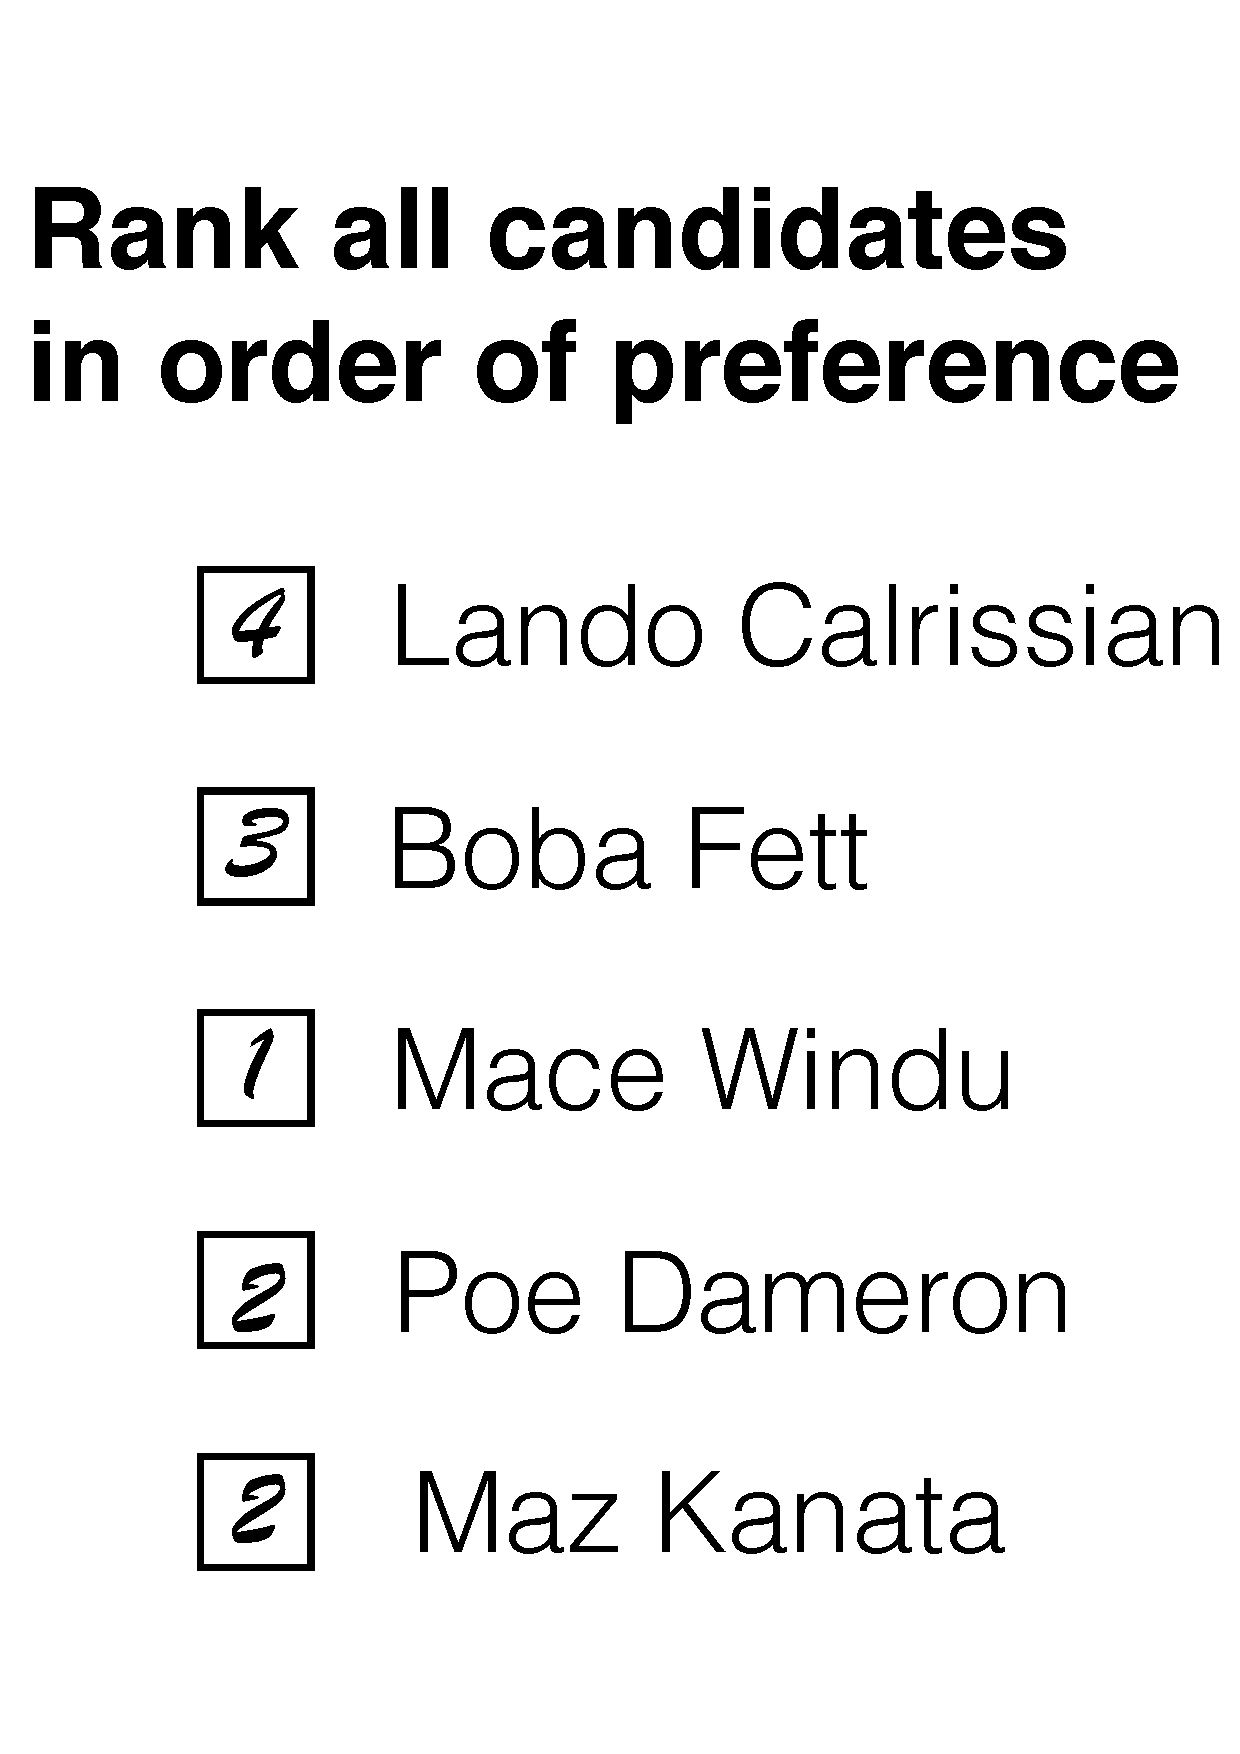
\includegraphics[scale=0.20]{bal-cropped.pdf}}
%%\end{center}
%%\end{frame}
%
%\begin{frame}
%\frametitle{Counting ballots}
%\lstfourth
%\end{frame}
%
%\begin{frame}
%\frametitle{All Schulze Election Have Winners}
%  \lsttwelve
%\end{frame}
%
%\begin{frame}
%\frametitle{Scrutiny Sheet}
%\begin{itemize}
%
%\item One major aspect of our work is that we are not only computing the set of winners, but in fact presenting
%\emph{evidence} for the fact that a particular
%candidate does or does not win. In the context of electronic vote counting, this is known as a \emph{scrutiny sheet}: a tabulation of all relevant data that allows
%us to verify the election outcome.
%
%\end{itemize}
%\end{frame}
%
%\begin{frame}
%\frametitle{Certificate}
%\lstnineth
%\end{frame}

%\begin{frame}
%\frametitle{Certificate}
%\lstfifth
%\end{frame}

%\begin{frame}
%\frametitle{Experimental result}
%{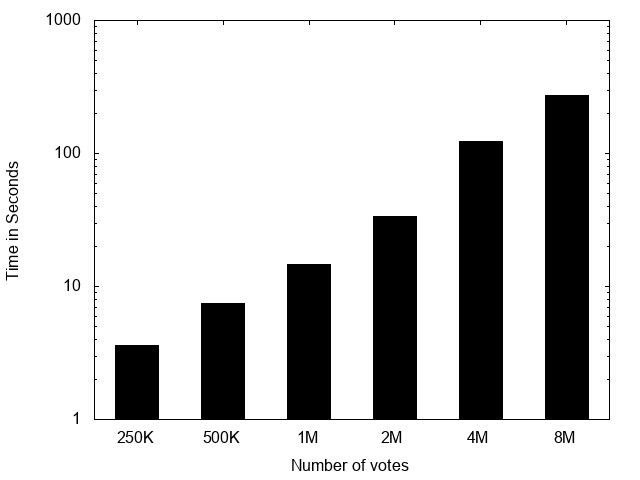
\includegraphics[scale=0.60]{with-cert.png}}
%\end{frame}



%\begin{frame}
%\frametitle{In Previous Presentation}
%\begin{itemize}
%\item Exploring the avenues of cryptography [July 2017 - December 2017]
%\item Risk limiting audit [January 2018 - June 2018]
%\item Connecting it with Helios [July 2018 - December 2018]
%\item Thesis writing [January 2019 - June 2019]
%\end{itemize}
%
%\end{frame}

%% New addition for september presentation
%\begin{frame}
%\frametitle{Problems ?}
%\begin{itemize}
%\item Problem with previous system is that ballots are in plaintext and it reveals 
%      all the information about ballots posted on bulletin board or certificate. 
%\item Can we achieve better way to count the ballots without revealing 
%	the content posted on bulletin board ? 
%\item Is it possible to convince the voter that we (Electoral Authority) have 
%	counted all the ballots honestly i.e we have included all the valid ballots 
%     and excluded all the invalid ballot in counting without revealing the content
%     of ballot itself ? \pause
%
%\item The answer is fortunately yes! Welcome to homomorphic encryption and zero 
%	knowledge proof.
%
%\end{itemize} 
%\end{frame}


%\begin{frame}
%\frametitle{Homomorphic Encryption and Zero Knowledge Proof}
%\begin{itemize}
%\item Homomorphic encryption is a form of encryption that allows computations to be carried out on ciphertext and generating an encrypted result. When encrypted result
%is decrypted, it matches the result of operations performed on the plaintext. 
%\item In additive Elgamal encryption, $E(m) = (g^r, g^m * h^r)$. We can easily 
%  	verify that $E(m_{1}) * E(m_{2}) = E (m_{1} + m_{2})$. 
%\item A zero-knowledge protocol is a method by which one party (the prover) can prove to another party (the verifier) that a given statement is true, without conveying any information apart from the fact that the statement is indeed true.
%\end{itemize} 
%\end{frame}

%\begin{frame}
%\frametitle{Enhancing the Security using Cryptography}
%\begin{itemize}
%\item The new representation of ballot is encrypted matrix, and we do point wise
%	multiplication of two encrypted ballots (matrices) to achieve the goal 
%	of addition in 	plain text.  \newline 
%	 Definition eballot := cand $\rightarrow$ cand $\rightarrow$ Z
%\item A ballot is valid if all the entries are either 0 or 1, and it has no
%	cycle. If voter prefers candidate $A$ over $B$ then it marks 1 in row 
%	$A$ and column $B$, and 0 in row $B$ and column $A$. However, a malicious 
%	user can mark ballot in such a way that it might lead to cycle, or inflate the 
%	ballot value of ballot. 
%
%\end{itemize} 
%\end{frame}
%
%\begin{frame}
%\frametitle{Enhancing the Security using Cryptography}
%\begin{itemize}
%
%\item The challenge in the counting process is  convincing the malicious user 
%	that your vote is invalid and discarded in final counting without decrypting 
%	his ballot, and convincing honest user that your vote is valid and included in 
%	final counting without decrypting his ballot.  
%	
%\item We pass the each encrypted ballot, u, through mix nets (secret permutation
% function), which permutes the ballot u and outputs encrypted ballot v with 
% zero knowledge proof data structure, zkp, that v is indeed the permutation of u.
% \item We decrypt the encrypted ballot v into plain text ballot b. We have formally 
% established that if b is valid (i.e. each entry is either 0 or 1, and there is no
% cycle) then ballot u is also valid.
%
%\end{itemize}
%\end{frame}

%\begin{frame}
%\frametitle{Computation as Inductive data type}
%\lstseventeen
%\end{frame}
%
%\begin{frame}
%\frametitle{Computation as Inductive data type}
%\lstthirteen
%\end{frame}
%
%\begin{frame}
%\frametitle{Computation as Inductive data type}
%\lstfourteen
%\end{frame}
%
%\begin{frame}
%\frametitle{Computation as Inductive data type}
%\lstfifteen
%\end{frame}
%
%\begin{frame}
%\frametitle{Computation as Inductive data type}
%\lstsixteen
%\end{frame}

%
%\begin{frame}
%\frametitle{Future Work}
%\begin{itemize}
%\item See all of you again in December of final presentation [December 2019]
%\item Risk limiting audit
%\item Verifying the cryptographic code
%\end{itemize}
%
%\end{frame}

\begin{frame}
\begin{center}
{\fontsize{40}{50}\selectfont Thank You!}
\begin{figure}
	\begin{center}
	
\includegraphics[scale=0.05]{turbo.jpg}
	\end{center}
  \end{figure}
\end{center}
\end{frame}

\end{document}
